%!TEX root = /Users/tcya/Dropbox/PhDthesis/thesis.tex

% \documentclass[journal=jpcbfk,manuscript=article]{achemso}
% \usepackage[version=3]{mhchem} % Formula subscripts using \ce{}


% \usepackage{tikz}
% \usetikzlibrary{arrows}
% \usepackage{natbib}
% \usepackage{graphicx}% Include figure files
% \usepackage{animate}
% \usepackage{dcolumn}% Align table columns on decimal point
% \usepackage{bm}% bold math

% \usepackage{animate}
% \usepackage{subfloat}
% \usepackage{amsmath} % AMS Math Package
% \usepackage{amsthm} % Theorem Formatting
% \usepackage{amssymb}	% Math symbols such as \mathbb
% %\nofiles

% \renewcommand{\labelenumi}{(\alph{enumi})} % Use letters for enumerate
% % \DeclareMathOperator{\Sample}{Sample}
% \let\vaccent=\v % rename builtin command \v{} to \vaccent{}
% \renewcommand{\v}[1]{\ensuremath{\mathbf{#1}}} % for vectors
% \newcommand{\gv}[1]{\ensuremath{\mbox{\boldmath$ #1 $}}}
% % for vectors of Greek letters
% \newcommand{\uv}[1]{\ensuremath{\mathbf{\hat{#1}}}} % for unit vector
% \newcommand{\abs}[1]{\left| #1 \right|} % for absolute value
% \newcommand{\avg}[1]{\left< #1 \right>} % for average
% \let\underdot=\d % rename builtin command \d{} to \underdot{}
% \renewcommand{\d}[2]{\frac{d #1}{d #2}} % for derivatives
% \newcommand{\dd}[2]{\frac{d^2 #1}{d #2^2}} % for double derivatives
% \newcommand{\pd}[2]{\frac{\partial #1}{\partial #2}}
% % for partial derivatives
% \newcommand{\pdd}[2]{\frac{\partial^2 #1}{\partial #2^2}}
% % for double partial derivatives
% \newcommand{\pdc}[3]{\left( \frac{\partial #1}{\partial #2}
%  \right)_{#3}} % for thermodynamic partial derivatives
% \newcommand{\ket}[1]{\left| #1 \right>} % for Dirac bras
% \newcommand{\bra}[1]{\left< #1 \right|} % for Dirac kets
% \newcommand{\braket}[2]{\left< #1 \vphantom{#2} \right|
%  \left. #2 \vphantom{#1} \right>} % for Dirac brackets
% \newcommand{\matrixel}[3]{\left< #1 \vphantom{#2#3} \right|
%  #2 \left| #3 \vphantom{#1#2} \right>} % for Dirac matrix elements
% \newcommand{\grad}[1]{\gv{\nabla} #1} % for gradient
% \let\divsymb=\div % rename builtin command \div to \divsymb
% \renewcommand{\div}[1]{\gv{\nabla} \cdot #1} % for divergence
% \newcommand{\curl}[1]{\gv{\nabla} \times #1} % for curl
% \let\baraccent=\= % rename builtin command \= to \baraccent
% \renewcommand{\=}[1]{\stackrel{#1}{=}} % for putting numbers above =

% %====commands for fermion operators =====
% %\newcommand{\cdup}[1]{c^\dagger_{#1\uparrow}}
% %\newcommand{\cdsig}[1]{c^\dagger_{#1\sigma}}
% %\newcommand{\cddown}[1]{c^\dagger_{#1\downarrow}}
% %\newcommand{\cup}[1]{c_{#1\uparrow}}
% %\newcommand{\csig}[1]{c_{#1\sigma}}
% %\newcommand{\cdown}[1]{c_{#1\downarrow}}
% %
% %
% %

% %%\listfiles

% \title{
% Intramolecular Charge and Energy Transfer Rates with Reduced Modes: Comparison to Marcus Theory for Donor-Bridge-Acceptor Systems
% }

% \author{Xunmo Yang}
% \affiliation{Department of Chemistry, University of Houston, Houston, TX 77204}


% \author{Eric R Bittner}
% \affiliation{Department of Chemistry, University of Houston, Houston, TX 77204}
% \phone{832-842-8849}
% \fax{713-743-2709}
% \email{bittner@uh.edu}





% \begin{document}

% %%%%%%%%%%%%%%%%%%%%%%%%%%%%%%%%%%%%%%%%%%%%%%%%%%%%%%%%%%%%%%%%%%%%%

% \begin{abstract}
%  We present a new, fully {\em ab initio} approach for computing intramolecular charge and
% energy transfer rates.  Using a time-convolutionless master equation approach and parameterized
% using couplings obtained using an accurate quantum chemical approach, we  benchmark the approach
% against  experimental results and Marcus theory rates for triplet energy transfer for a
% series of donor-bridge-acceptor systems.
% An important component of our analysis is the use of a projection operator scheme
% that parses out specific internal nuclear motions that accompany
% the electronic transition.
% Using an iterative Lanczos approach, we  concentrate the coupling between the electronic and nuclear
% degrees of freedom into a small number of reduced harmonic modes.
% We find that  using only a single reduced mode--termed the ``primary mode'',
%  one obtains an accurate evaluation of the golden-rule rate constant and
% insight into the nuclear motions responsible for coupling the initial and final electronic states.
% In particular, the primary mode reflects the irreducible representation of the
% donor and acceptor excited states.
% \end{abstract}

% {\bf Keywords:} Quantum master equation, energy transfer rates, diabatic states,  triplet energy transfer

% \newpage

\chapter{Benchmark and Primary Mode}\footnotetext{Part of this chapter has been published in Xunmo Yang and E. R. Bittner, Intramolecular Charge- and Energy-Transfer Rates with Reduced Modes: Comparison to Marcus Theory for Donor–Bridge–Acceptor Systems. The Journal of Physical Chemistry A\textbf{118}, 5196 (2014)}\label{chap:chapt2}
\section{Introduction}
\label{sec:intro}

% Energy and electronic transport plays a central role in a
% wide range of  chemical  and biological systems.
% It is the fundamental mechanism for transporting the  energy  of a
% absorbed photon to a reaction center in light harvesting systems
% and for initiating a wide range of photo-induced  chemical processes,
% including vision, DNA mutation, and pigmentation.
% The seminal model for calculating electron transfer rates was developed by
% Marcus in the 1950's\cite{marcus1956theory,marcus1965theory,marcus1993electron}.
% \begin{equation}
% k_{Marcus}=\frac{2\pi}{\hbar}|V_{ab}|^{2}\frac{1}{\sqrt{4\text{\ensuremath{\pi}}k_{B}T\lambda}}e^{-(\lambda+ \Delta\epsilon)^{2}/4\text{\ensuremath{\lambda}}k_{B}T}.\label{eq:marcus}
% \end{equation}
% where $\lambda$ is  energy required to reorganize the environment
% following the transfer of an electron from donor to acceptor.
% and $\Delta \epsilon$ is the driving force for the reaction.

% \begin{figure}[h]
% 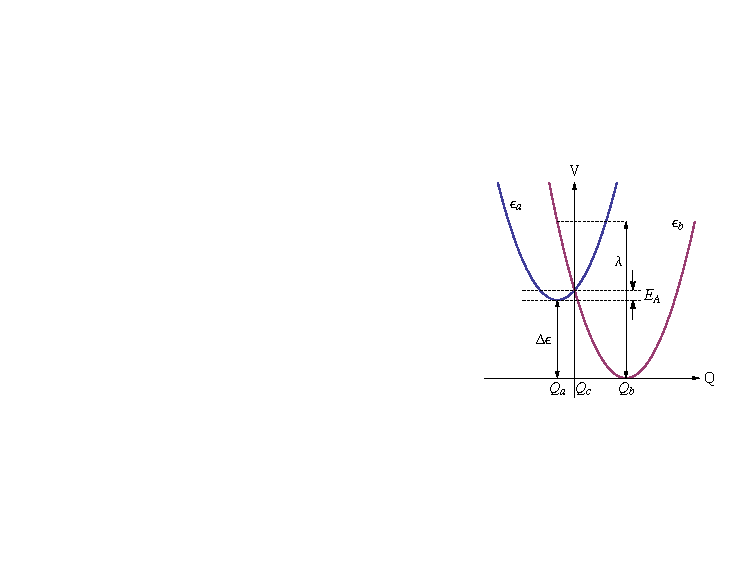
\includegraphics[width=0.5\columnwidth]{Chapters/chap2/Figure1}
% \caption{Sketch of Marcus parabolas for a model energy or charge transfer system.
% Labeled are the key parameters used to compute the Marcus rate constant (Eq. \ref{eq:marcus}).
% Energies are given in eV and the collective nuclear displacement  is dimensionless.
% }
% \label{marcus}
% \end{figure}


% If we assume that the nuclear motions about the equilibrium configurations of the
% donor and acceptor species is harmonic,  the chemical reactions resulting from
% energy or charge transfer events can be understood in terms of intersecting
% diabatic potentials as sketched in Fig.~\ref{marcus}.    The upper and lower
% curves are the adiabatic potential energy surfaces describing the nuclear dynamics
% resulting from an energy or charge transfer event, taking the geometry of the donor
% state as the origin.
% %For reactions carried out in open systems,  the Marcus parabolas represent
% %free energy surfaces with driving force $\Delta G$.
% As the transfer occurs by crossing an energy barrier,
% the transfer rate can be expected to be in the Arrhenius form
% \begin{eqnarray}
% k\propto e^{-E_{A}/k_{B}T},
% \end{eqnarray}
% with $E_{A}$ as the activation energy.
%  Using $E_{A}={(\lambda+\Delta \epsilon)^{2}}/{4\lambda}$
%  we can relate the activation energy to both the reorganization energy and driving force, $-\Delta \epsilon$.
% One of the most profound predictions of the theory is that  as the driving force increases,
% the transfer rate reaches a maximum and further increases in the driving force
% lead to lower reaction rates, termed the inverted regime.



In this chapter we focus on the rates of triplet exchange between a naphthalene donor and a benzaldehyde acceptor linked by a variety of bridging units.
\begin{center}
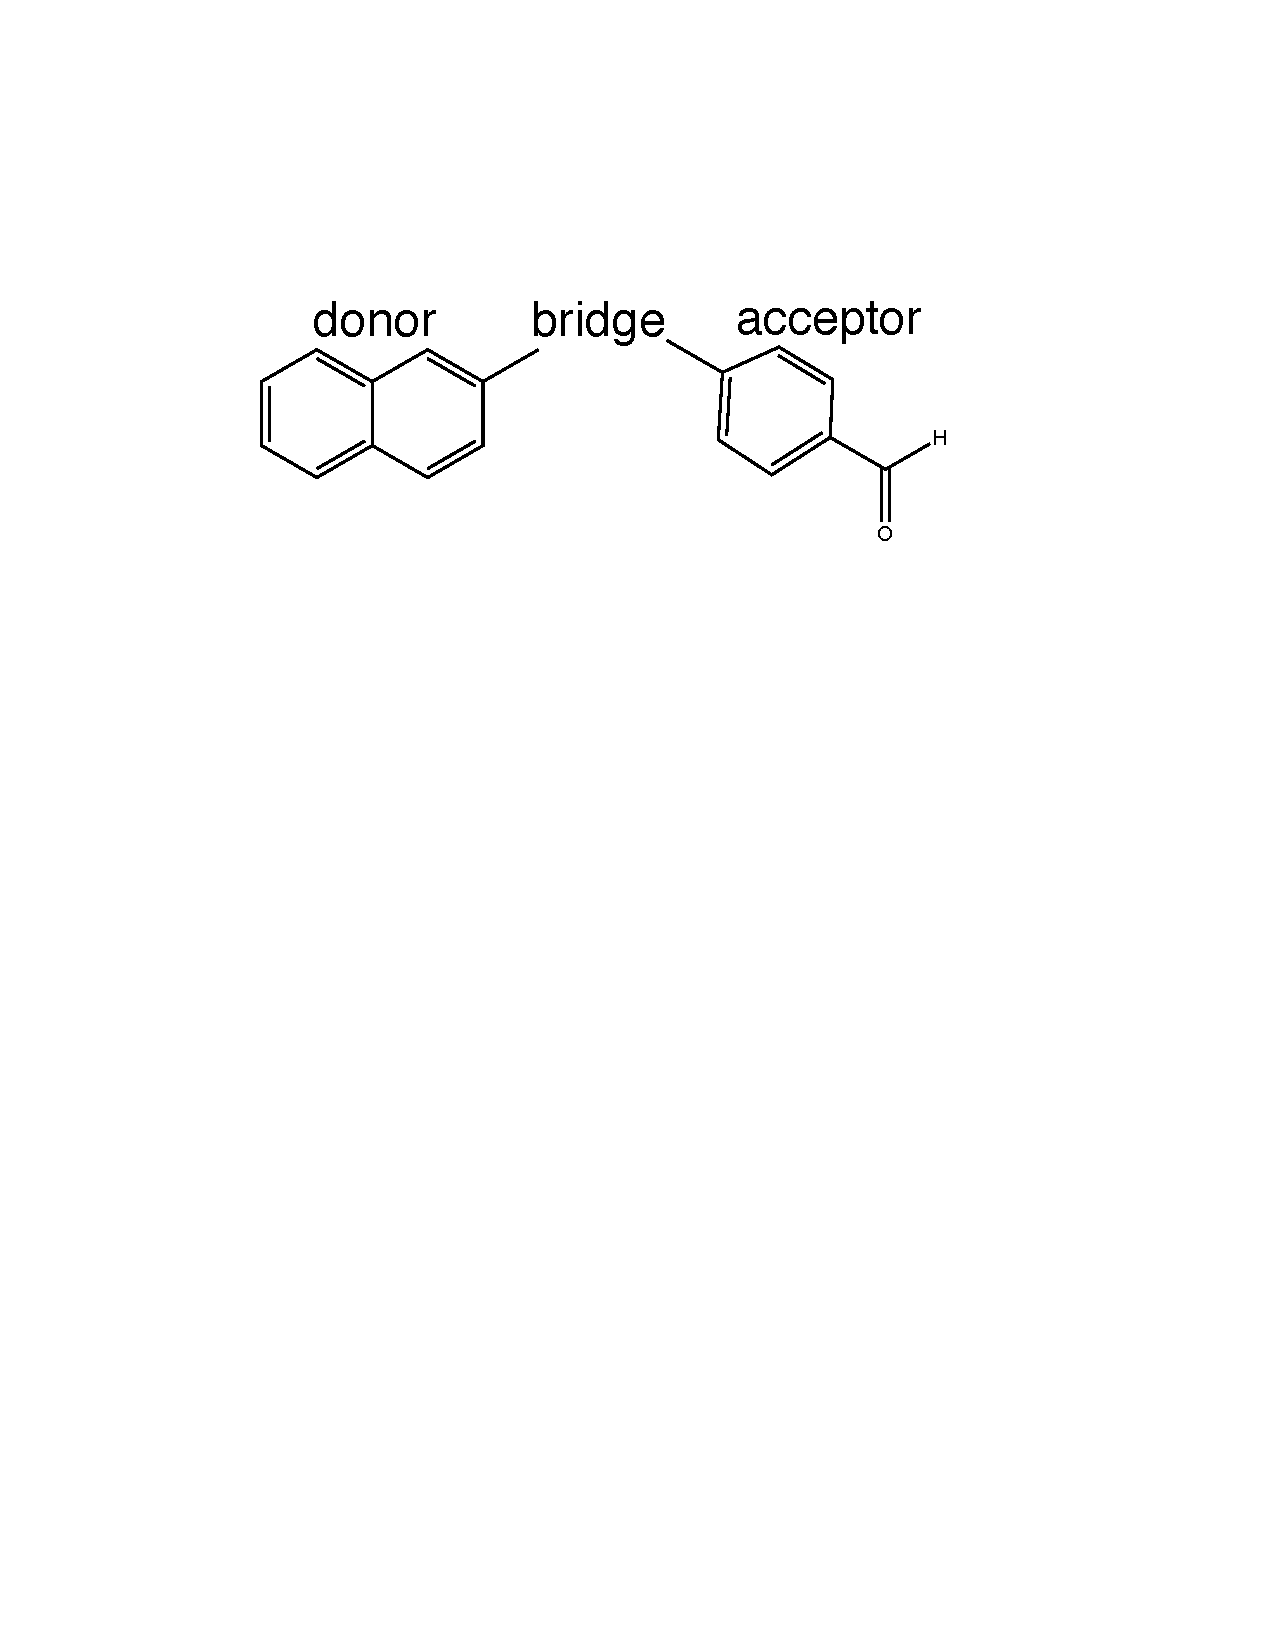
\includegraphics[width=0.50\columnwidth]{Chapters/chap2/Scheme1}
\end{center}
Triplet energy exchange in these systems occurs via the through-space Dexter mechanism \cite{dexter1953theory}.
This is a short-ranged interaction involving the simultaneous exchange of two electrons between the
donor and acceptor moieties.
Systems such as these formed the basis of a series of experiments by  Closs and Miller \cite{miller1984intramolecular}
in which they verified the existence of the Marcus ``inverted regime'' - the very negative $\Delta G$ domain where transfer becomes slower -
and serve as crucial benchmarks for testing new theoretical models for computing
energy and charge transfer rates \cite{subotnik2008constructing,subotnik2009initial,subotnik2010predicting}. The molecules are sketched in Table. \ref{summarytable}.

The chapter is arranged in this way. First we examine the validity of the assumptions in our method. Then we apply the method to obtain theoretical transfer rate constants, and compare these to experimental results. Finally, we use the projection scheme to find the primary modes in the reactions.
% The modes turn out to show certain symmetry.


% A number of years ago,  we developed a time-convolutionless  master equation approach for computing
% state-to-state rates in which the coupling between  states depends upon the
% nuclear coordinates\cite{pereverzev2006time}. This approach incorporates a fully quantum
% mechanical treatment of both the nuclear and electronic degrees of freedom and recovers
% well-known Marcus expression in the semiclassical limit.  The model is parameterized by the
% vibrational normal mode frequencies, and the electronic energies and energy derivatives
% at a reference configuration.  The approach has been used by our group to compute state-to-state
% transition rates in semi-empirical models for organic semiconducting light-emitting diode and photovoltaics
% \cite{tamura2008phonon,tamura2007exciton,bittner2014noise,singh2009fluorescence}.
% This paper represents the first time we have used this approach within the context of a fully {\em ab initio} quantum
% chemical model.   As such, this present work provides an important benchmark of the approach since all parameters will be determined
% using state-of-the-art quantum chemical methods
% and results compared to both theoretical and experimental
% rates.

% Central to the work presented here is the use of a diabatization scheme for determining
% donor and acceptor states in a molecular unit.  We benchmark the approach
% by computing the  triplet energy transfer rates for a series of donor-bridge-acceptor molecules
% originally studied by Closs\cite{miller1984intramolecular}.  The triplet energy transfer rates computed using our approach
% compare well against both the experimental rates and with
% more recent theoretical rates presented by Subotnik {\em et al.}
% \cite{subotnik2008constructing,subotnik2009initial,subotnik2010predicting}.
% An important component of our analysis is the use of a projection operator scheme
% that parses out specific internal nuclear motions that accompany
% the electronic transition.
% Similar decomposition schemes have been presented by Burghardt
%  \cite{cederbaum2005short,gindensperger2006shortI,gindensperger2006shortII,cederbaum2005short}
%  and the approach used here builds upon the method given in Ref.~\cite{pereverzev2009energy}.
%  By analyzing the electron-phonon couplings, we can
% discern a reduced set of motions that are responsible for coupling between the donor and
% acceptor states.



% \section{Theoretical Approach}

% \subsection{Model Hamiltonian}
% We consider a generic model for $n$ electronic states coupled linearly
% to a phonon bath.  Taking the electronic ground state of the system as a reference
% and assuming that the electronic states are coupled linearly to a common set of
%  modes, we arrive a generic form for the Hamiltonian:
%  \begin{eqnarray}
% H=\left(\begin{array}{cc}
% \epsilon_{1} & 0\\
% 0 & \epsilon_{2}
% \end{array}\right)+\left(\begin{array}{cc}
% {\mathbf g}_{11}&{\mathbf g}_{12} \\
% {\mathbf g}_{21} &{\mathbf g}_{22}
% \end{array}\right)\cdot{\mathbf q} +\frac{{\mathbf p}^{2}}{2}+\frac{1}{2}\mathbf{q}^{T}\cdot\mathbf\Omega\cdot\mathbf{q}.
% \nonumber \\
% \label{ham1}
% \end{eqnarray}
% Here, the first term contains the electronic energies, $\epsilon_{1}$ and $\epsilon_{2}$ computed at a
% reference geometry--typically that of the donor or acceptor state.   The second term represents the
% linearized coupling between the electronic and nuclear degrees of freedom given in terms of the mass-weighted
% normal coordinates $\mathbf q$.   The diagonal terms
% give the adiabatic displacement forces between the reference geometry and the two states.  If we choose one of the
% states as the reference state, then either $\mathbf g_{11}$ or $\mathbf g_{22}$ will vanish.
% The remaining two terms correspond to the harmonic motions of the nuclear normal modes, given here in mass-weighted normal coordinates.
% In the normal mode basis, $\mathbf \Omega$  is diagonal with elements corresponding to the normal mode frequencies, $\omega_{j}^{2}$.


% We now separate Eq.~\ref{ham1} into diagonal and
% off-diagonal terms
% \begin{eqnarray}
% \hat  H = \hat H_{o} + \hat V
% \end{eqnarray}
% and perform a polaron transform
% using the unitary transformation~\cite{grover1970exciton,rice1994excitons,pereverzev2006time}.
% \begin{eqnarray}
% U&=&e^{-\sum_{ni}\!\!\frac{g_{nni}}{\hbar\omega_i}|n\rangle \langle
% n|(a^{\dagger}_i-a_i)}
%  \nonumber \\
% &=&
% \sum_{n}|n\rangle \langle n|e^{-\sum_{i}\!\!\frac{g_{nni}}{\hbar\omega_i}(a^{\dagger}_i-a_i)}
% \label{unitary}
% \end{eqnarray}
% under which the transformed Hamiltonian is written in terms of the
% diagonal elements
% \begin{eqnarray} \tilde H_0=U^{-1}H_0U
% =\sum_n\tilde\epsilon_n |n\rangle \langle
% n|+\sum_i\omega_ia^{\dagger}_ia_i,
%  \end{eqnarray}
% with  the renormalized electronic energies,
% \begin{eqnarray}
% \tilde\epsilon_n=\epsilon_n-\sum_{i}\frac{g_{nni}^2}{\hbar\omega_i},
% \end{eqnarray}
% and off-diagonal terms,
% \begin{eqnarray} \hat V_{nm}=\sum_{i}g_{nmi}\left(a^{\dagger}_i+
% a_i-\frac{2g_{nni}}{\hbar\omega_i}\right)e^{\sum_{j}\frac{(g_{nnj}-g_{mmj})}{\hbar\omega_j}(a^{\dagger}_j-a_j)}.
% \label{opm}
% \end{eqnarray}
% In the transformed (or dressed) picture the electronic transition from state
% $|n\rangle$ to $|m\rangle$ is accompanied by the excitations of all the
% normal phonon modes.  Transforming to the interaction representation
% and performing a trace over the phonons gives the spectral density in
% terms of the autocorrelation of the electron-phonon coupling
% operators.
% \begin{eqnarray}
% S_{nm}(\tilde\omega) = \int_{-\infty}^{\infty} dt e^{-i\tilde \omega t}\langle \hat V_{nm}(t) \hat V_{mn}(0)\rangle.\label{spec-dens}
% \end{eqnarray}
% Here, $\hat V_{nm}(t)$ is the electron-phonon coupling term in the Heisenberg representation and
% $\langle \cdots \rangle$ denotes a thermal average over the
% vibrational degrees of freedom.
% The derivation and explicit form for the kernel in Eq.~\ref{spec-dens}  is quite lengthy and is given in
% Ref.~\cite{pereverzev2006time}.

% \subsection{Non-Markovian Master Equation and Golden-Rule rates}

% In Ref.~\cite{pereverzev2006time}, Pereverzev and Bittner derived
% a non-Markovian, time-convolutionless form of the Pauli master
% equation (TCLME)  for general system described by Eq.~\ref{ham1}.
% \begin{eqnarray}
% \frac{dP_{n}}{dt} = \sum_{m} W_{nm}(t)P_{m}(t) - \left(\sum_{m} W_{mn}(t)\right)P_{n}(t)
% \end{eqnarray}
% where the time-dependent rates are given by
% \begin{eqnarray}
% W_{nm}(\tau)=2{\rm Re}\int_{0}^{\tau}dt\left\langle \hat V_{nm}(0)\hat V_{mn}\left(t\right)\right\rangle e^{-i\tilde\omega_{nm}t}.
% \label{rate-expression}
% \end{eqnarray}
% In the limit that $\tau\to\infty$, Eq.~\ref{rate-expression} gives the Fermi's Golden Rule expression for the
% transition rate,
% \begin{eqnarray}
% k_{nm}=2{\rm Re}\int_{0}^{\infty}dt\left\langle \hat V_{nm}(0)\hat V_{mn}\left(t\right)\right\rangle e^{-i\tilde\omega_{nm}t}.
% \label{gr-expression}
% \end{eqnarray}

% At this point it is useful to connect the various terms in the phonon-dressed Hamiltonian
% with specific physical parameters.
% First, the reorganization energy is given by
% %The terms involving $$
% %are related to the reorganized energy difference between the two states.
% %$$
% %\lambda_{nm} =\sum_{j}((g_{nnj}-g_{mmj})/\omega_j)^{2} = \sum_{j}\hbar \omega_{j}S_{j}
% %$$
% \[
% \lambda_{nm}=\sum_{j}\frac{\left(g_{nnj}-g_{mmj}\right)^{2}}{\omega_{j}} = \sum_{j}\hbar \omega_{j}S_{j}
% \]
% where  the $\{S_{j}\}$  are  the Huang-Rhys factors for each phonon mode.
% These are related to the Franck-Condon factor
% describing the overlap between the $v_j=1$ vibronic state in one electronic state
% with the $v_j=0$ vibronic state in the other.
% Likewise, the energy difference between the renormalized energy gaps is related to the
% driving force of the state-to-state transition,
% \begin{eqnarray}
% \Delta E_{nm} = \tilde \epsilon_n-\tilde \epsilon_m.
% \end{eqnarray}


% The difficulty in using this approach is that
% it requires both diagonal (${\mathbf g}_{nn}$) and off-diagonal  (${\mathbf g}_{nm}$) derivative couplings between
% adiabatic states.    In the following section, we discuss how we have used the Edmiston-Ruedenberg localization scheme
% to estimate the couplings\cite{edmiston1963localized}.   We also
% present how one can construct a reduced set of harmonic modes that
% fully capture the electron/nuclear coupling.
% \subsection{Parameterization From Quantum Chemistry}

%  In order to obtain the final form of our target Hamiltonian, we assume the diabatic  potentials
% are a good approximation to the actual adiabatic potentials.

% When the adiabatic (and diabatic) energy minima
% are far enough away from the crossing points and the mixing angles between the diabatic  and adiabatic
% states is small, we can
% use the gradients of the adiabatic potentials to approximate the diabatic potentials.
% Thus, if we perform calculations at the
% optimized geometry of the final acceptor state  ({\em i.~e.} about $Q_{2}$  in Fig.~\ref{marcus}),
% we can write the Hamiltonian as
% \begin{eqnarray}
% H_{dia,e}=\left(\begin{array}{cc}
% \epsilon_{1} & V_{12}\\
% V_{21} & \epsilon_{2}
% \end{array}\right)+\left(\begin{array}{cc}
% 0 & 0\\
% 0 & 1
% \end{array}\right) {\mathbf g}_{22}\cdot{\mathbf q}+H_{osc},
% \end{eqnarray}
% where $H_{osc}$ is the harmonic oscillator Hamiltonian for the vibrational normal modes.
% The linear assumption amounts  to performing a series expansion of the
% full, multi-dimensional coupling term and keeping only the lowest order terms.
% Systematic improvement can be made by including higher-order (e.g.  quadratic) off-diagonal couplings.
% However, this would involve a substantial increase in the complexity of the theory.
% The linear assumption is reasonable so long as  the mixing angle is small,
% as verified by the benchmark calculations presented below.

% We obtain the diabatic couplings $V_{12}$
% and the mixing angle $\theta$  via ER localization and transform the electronic Hamiltonian
% from the adiabatic basis to the diabatic basis {\em viz.}
% \begin{equation}
% H_{dia}=\left(\begin{array}{cc}
% \cos\theta & -\sin\theta\\
% \sin\theta & \cos\theta
% \end{array}\right)\left(\begin{array}{cc}
% \epsilon_{1}  & 0 \\
% 0  & \epsilon_{2}
% \end{array}\right)\left(\begin{array}{cc}
% \cos\theta & \sin\theta\\
% -\sin\theta & \cos\theta
% \end{array}\right).\label{eq:boys}
% \end{equation}
% The diabatic coupling is then given by
% \begin{eqnarray}
% V_{ab}=\frac{1}{2}\sin2\theta\left(\epsilon_{2}-\epsilon_{1}\right).
% \end{eqnarray}


% We then diagonalize the electronic part and transform the electron/nuclear coupling
% back into the adiabatic basis.  In doing so,  we obtain the Hamiltonian in the
% form given in Eq. \ref{ham1}
% \begin{eqnarray}
% H&=&U^{T}H_{dia}U\nonumber  \\
% &=&\left(\begin{array}{cc}
% E_{1}  & 0 \\
% 0 & E_{2}
% \end{array}\right)+\left(\begin{array}{cc}
% \sin^{2}\theta & \frac{1}{2}\sin2\theta\\
% \frac{1}{2}\sin2\theta & \cos^{2}\theta
% \end{array}\right) {\mathbf g}_{22}.{\mathbf q} \nonumber \\
% &+& H_{osc}.\label{eq:locaiHam}
% \end{eqnarray}

\section{Assumption Validity}

Our method employs two assumptions. First is that the diabatic surfaces are harmonic. Second, the Condon approximation is valid, namely, the diabatic couplings are independent of nuclear coordinates in the region where the reaction occurs.
In Fig.~\ref{parabs} we show the computed adiabatic potential curves and off-diagonal couplings along an interpolation coordinate
connecting the equilibrium geometries of the donor and acceptor states for the d-2,6ae molecule.
The dashed curve gives the parabolic approximation to the
lower potential curves.  Along this coordinate, the off-diagonal coupling is small and essentially linear and the parabolic
approximation provides a good approximation to the actual potential.  This indicates that the assumptions in our model Hamiltonian
are generally robust for the systems we consider herein.

\begin{figure}[!ht]
\subfloat[c-1,4ee]{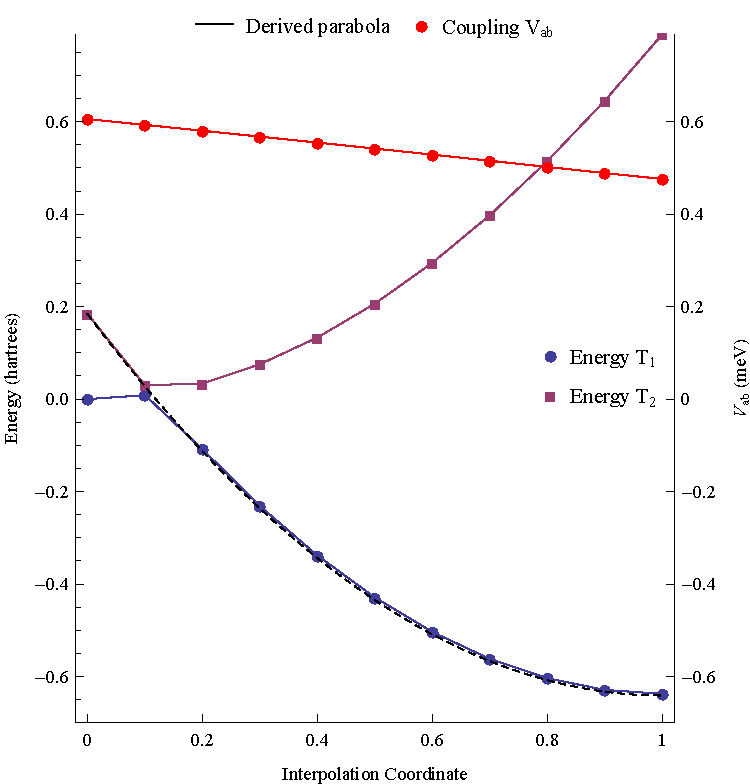
\includegraphics[width=0.45\columnwidth]{Chapters/chap2/Figure2a}}
\subfloat[d-2,6ae]{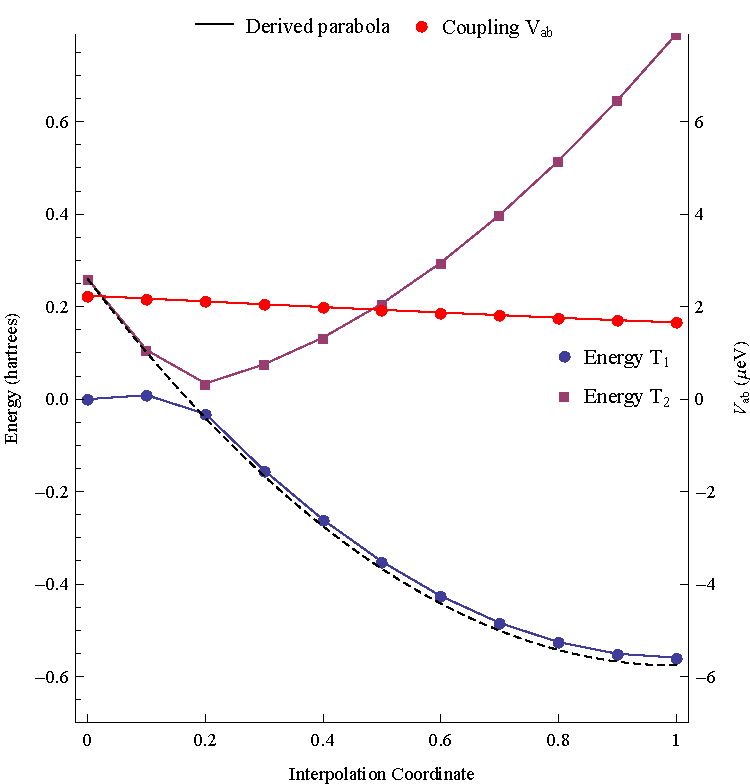
\includegraphics[width=0.45\columnwidth]{Chapters/chap2/Figure2b}}
\caption{Adiabatic energy curves and off-diagonal couplings computed along an interpolation coordinate between the
$D^{*}-B-A$ and $D-B-A^{*}$ equilibrium geometries.  $V_{ab}$ is the off-diagonal coupling at each point along this coordinate.} \label{parabs}
\end{figure}





\section{Energy transfer rates in  Donor-Bridge-Acceptor systems}


Using the ER localization approach explained in Section \ref{sec:ER}, all parameters needed for our model can be  obtained from
standard  quantum chemical packages.   The vertical energies, $\epsilon_{a}$
and $\epsilon_{b}$ are obtained from single point CI(S) calculations at a given
reference geometry.   We then project the energy gradients onto the vibrational normal
coordinates to obtain the electron-phonon coupling constants.  Either the Boys or ER
localization scheme can be use to compute the mixing
angles for constructing diabatic states. For all calculations shown here we
used the Q-Chem 4.0 \cite{QCHEM4} code and employed the 6-31G(d){*}{*} basis set
in order to compare our results  against other theoretical results in  Ref.~\cite{subotnik2010predicting}.

 We  benchmark our approach against a series of donor-bridge-acceptor
molecules studied by Closs \cite{closs1988determination,closs1988intramolecular,closs1989connection}.
These cases are significant in that they provided a crucial verification of the Marcus inverted regime.
Table~\ref{summarytable} and Fig.~\ref{compare}  summarize our results.
In addition, we give the diabatic coupling $V_{ab}$, reorganization energy $\lambda$, and driving force $\Delta \epsilon$
computed using the Edmiston-Reudenberg (ER) localization method.

\begin{sidewaystable}
% \begin{table*}[t]
\begin{centering}
\begin{tabular}{llccc|ccc}
\hline \hline
 & & \multicolumn{3}{c}{Rates (s$^{-1}$) }& \\
                &                                                                &   Expt.                 &        Marcus Theory   & This work      & \multicolumn{3}{c}{Marcus theory parameters} \\
 Bridge   &  Structure                                                &        Ref.~\cite{closs1988determination,closs1989connection} &              Ref. \cite{subotnik2010predicting}  &                  &      $\lambda$ (eV)  &  $\Delta \epsilon$ (eV)  &  $V_{ab}$ ($\mu$eV) \\
\hline
 c-1,3ea  &  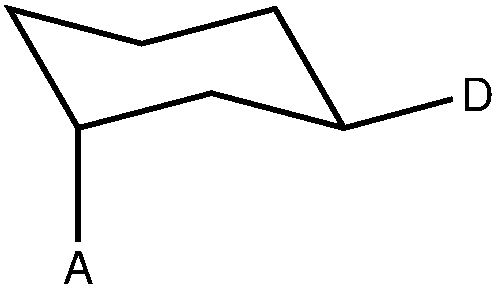
\includegraphics[height=.60cm,width=2cm]{Chapters/chap2/Table1-c13ea.pdf}  &                     3.3E9  &                     3.9E9  &          2.2E9  &           0.823  &           -0.612  &      470.1  \\
\hline
 c-1,3ee  &  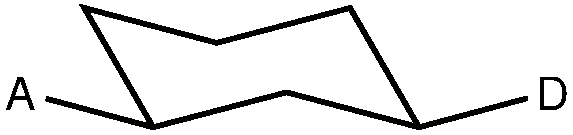
\includegraphics[height=0.4cm,width=2cm]{Chapters/chap2/Table1-c13ee.pdf}  &                     7.7E9  &                    2.1E10  &         2.8E10  &           0.810  &           -0.580  &     1687.3  \\
\hline
 c-1,4ea  &  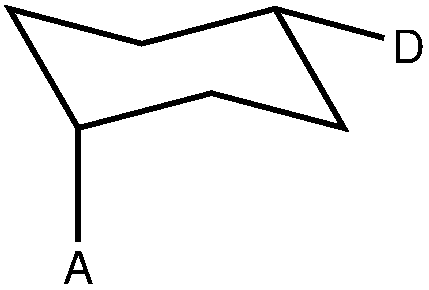
\includegraphics[height=0.6cm,width=2cm]{Chapters/chap2/Table1-c14ea.pdf}  &                     4.0E7  &                     1.3E7  &          1.8E7  &           0.817  &           -0.604  &      43.20 \\
\hline
 c-1,4ee  &  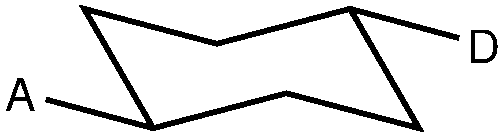
\includegraphics[height=0.4cm,width=2cm]{Chapters/chap2/Table1-c14ee.pdf}  &                     1.3E9  &                     3.9E9  &          3.6E9  &           0.826  &           -0.642  &      605.8  \\
\hline
 d-2,6ae  &  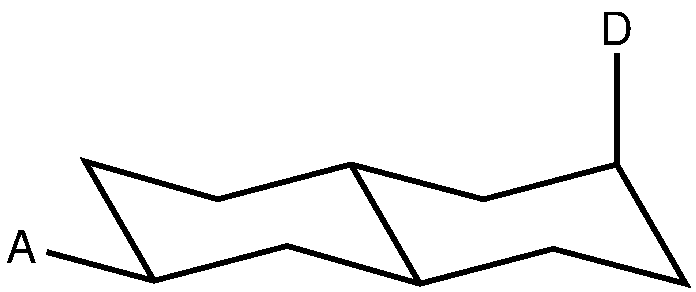
\includegraphics[height=0.6cm,width=2cm]{Chapters/chap2/Table1-d26ae.pdf}  &                     1.3E5  &                     1.0E4  &          4.7E4  &           0.836  &           -0.577  &    2.239  \\
\hline
d-2,6ea  &  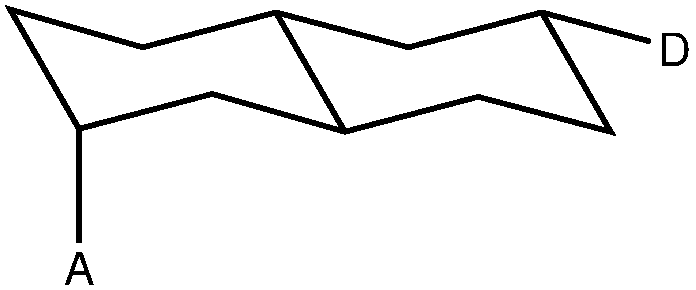
\includegraphics[height=0.6cm,width=2cm]{Chapters/chap2/Table1-d26ea.pdf}  &                     7.0E5  &                     3.9E4  &          5.8E4  &            0.821  &            -0.609  &    2.414  \\
\hline
 d-2,6ee  &  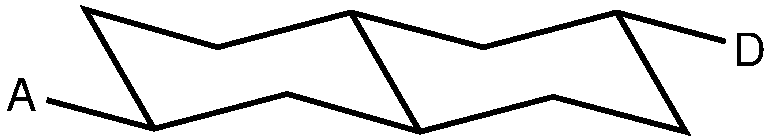
\includegraphics[height=0.4cm,width=2cm]{Chapters/chap2/Table1-d26ee.pdf}  &                     3.1E6  &                     5.0E6  &          4.8E6  &           0.810  &           -0.581  &     22.12  \\
\hline
 d-2,7ae  &  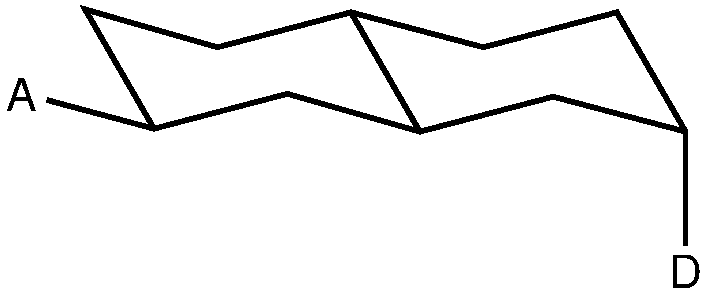
\includegraphics[height=0.6cm,width=2cm]{Chapters/chap2/Table1-d27ae.pdf}  &                     1.1E7  &                     2.8E7  &          3.0E7  &           0.826  &           -0.605  &     55.16   \\
\hline
 d-2,7ea  &  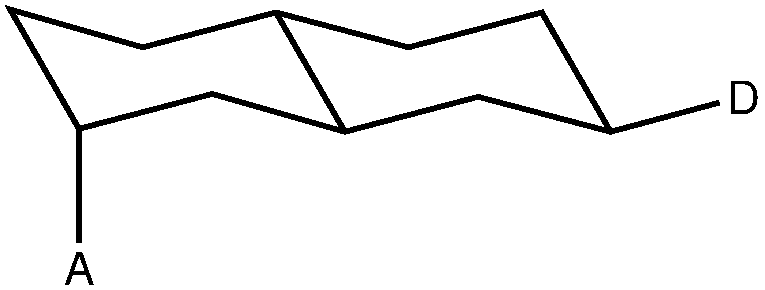
\includegraphics[height=0.6cm,width=2cm]{Chapters/chap2/Table1-d27ea.pdf}  &                     1.5E7  &                     1.8E7  &          4.3E7  &           0.817  &           -0.605  &     65.85  \\
\hline
 d-2,7ee  &  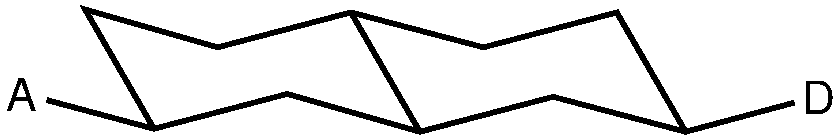
\includegraphics[height=0.4cm,width=2cm]{Chapters/chap2/Table1-d27ee.pdf}  &                     9.1E7  &                     3.5E8  &          3.4E8  &           0.831  &           -0.648  &     185.1  \\
\hline
 M        &  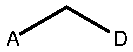
\includegraphics[height=0.4cm,width=2cm]{Chapters/chap2/Table1-M.pdf}      &                    5.0E10  &                      n.r.  &          1.2E9  &              0.896  &      -0.636  &      357.0 \\
\hline
\end{tabular}

\par\end{centering}
\caption{Comparison of triplet-triplet energy transfer rates obtained from our  approach,  Marcus rates are
from ~Ref. \cite{subotnik2010predicting}
and experimental rates from Refs. \cite{closs1988determination,closs1989connection}.   The experimental error is estimated to be 20\% in each
case studied here.
The $V_{ab}$ are the diabatic couplings obtained using  Edmiston-Ruedenberg diabatization.
In each case, D =4-benzophenonyl and A = 2-napthyl.  n.r. = Not Reported.
}
\label{summarytable}
% \end{table*}
\end{sidewaystable}



\begin{figure}[t]
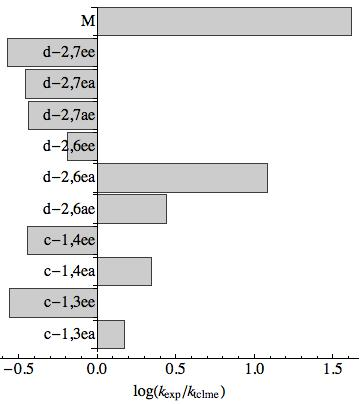
\includegraphics[width=0.5\columnwidth]{Chapters/chap2/Figure3}
\caption{Comparison between predicted (TCLME) rate constants and the experimental rates from ~Ref. \cite{miller1984intramolecular}.  With exception of
the methyl and D-2,6-ea bridged cases, the TCLME results are in good agreement with the experimental results.  }\label{compare}
\end{figure}


In general, our results and those in ~Ref. \cite{subotnik2010predicting} agree with each other well and both are
comparable to the experimental results which report an estimated error of 10-20\% in the
rate for each case presented here.  Furthermore,  all theoretical values were computed
in the absence of solvent environment, whereas the experiments were all performed in benzene solvent at a standard temperature.
However,  there is considerable disagreement between the experimental and theoretical results for
the d-2,6ea and methyl (M) bridged cases.   For the d-2,6ea bridge,  our results are similar to the
Marcus theory rates given in Ref. \cite{subotnik2010predicting}.  In this case, the
 the ER localization gives a  small diabatic coupling
 % $V_{ab} = 4.4\times 10^{-6}$eV
 and it was  difficult to obtain converged localized states.
In the case of the methyl-bridge,  there is a significant change in the geometry between donor and acceptor states.
As a result,  the potential surfaces are no longer parabolic
and the Condon approximation breaks down \cite{subotnik2010predicting}.








% \section{Determining the Optimal Electron-Phonon Coupling Components}

% While the Marcus expression is elegant in its simplicity in requiring three parameters that
% can be obtained experimentally, it masks a wealth of detail that underlie the quantum transition.
% Central to the theory is that there exists a collective nuclear displacement coordinate
% that connects the initial geometry of the donor to the final geometry of the acceptor.

% Generally speaking, this collective coordinate involves all nuclear degrees of freedom.
% However, the form of the electronic Hamiltonian in Eq.~\ref{ham1} suggests that
% there exists a subset of motions that are specific modes  that capture the majority of the
% electronic/nuclear coupling and give the dominant contribution to the collective
% reaction coordinate.  Within the linearized approximation for the electronic/nuclear coupling,
% we can write a force tensor
% \begin{eqnarray}
% {\mathbf F} =
% \left(\begin{array}{cc}
% {\mathbf g}_{11}&{\mathbf g}_{12} \\
% {\mathbf g}_{21} &{\mathbf g}_{22}
% \end{array}\right)
% \end{eqnarray}
% where ${\mathbf F}\cdot \mathbf q$ is the electronic/nuclear coupling term in Eq.~\ref{ham1}.
% If we consider each unique element $\{ \mathbf g_{11}, \mathbf g_{12} , \mathbf g_{22}\}$ to be
% linearly independent, but non-orthogonal force vectors,  one can develop a  projection operator scheme to
% to parse the $N$-dimensional linear vector space spanned by the mass-weighted normal mode vectors into two subspaces:
% one spanned by three vectors describing the coupling between the electronic states
% and the other spanned by the remaining $N-3$ dimensional space spanned by motions that
% do not couple the electronic states.
% This  subspace  can be generated by defining a projection operator
% \begin{eqnarray}
% \mathbf{P}=\sum_{\alpha\beta}'\left(\mathbf{S^{-1}}\right)_{\alpha\beta}\mathbf{g_{\alpha}}\otimes\mathbf{g_{\beta}}
% \end{eqnarray}
% in which the summation is limited to linearly independent vectors.
%    Here $\mathbf{S}_{\alpha\beta}=\mathbf{g_{\alpha}}\cdot\mathbf{g_{\beta}}$,
% $\otimes$ is outer product,  and $\mathbf{I}$ is unitary operator.
% This $N\times N$ matrix projects out all normal modes that are directly coupled to the
% electronic degrees of freedom and
%  its complement $\mathbf{Q}=\mathbf{I}-\mathbf{P}$ projects out all modes not directly coupled.
% By diagonalizing the matrix
% \begin{eqnarray}
% \mathbf{K}=\mathbf{P}\cdot\mathbf\Omega\cdot \mathbf{P}+\mathbf{Q}\cdot\mathbf\Omega\cdot\mathbf{Q}
% \end{eqnarray}
% we obtain a  transformation, ${\mathbf M}$,  between the normal coordinates and a new set of orthogonal
% coordinates.  Both $\mathbf{P}\cdot\mathbf\Omega\cdot \mathbf{P}$ and $\mathbf{Q}\cdot\mathbf\Omega\cdot\mathbf{Q}$ are $N\times N$ matrices.
% However, for a two-state system, the former will have exactly $3$ non-trivial eigenvalues, $\{\alpha_{p}\}$, with corresponding
% eigenvectors, $\{ M_{p}\}$, whereas the latter will have exactly $N_{r} = N-3$ non-trivial eigenvalues, $\{\alpha_{q}\}$,  and corresponding
% eigenvectors, $\{M_q\}$.   This the full $N\times N$ transformation is formed by joining the non-trivial vectors from the
% two respective subspaces ${\mathbf M} = \{M_{p}, M_{q}\}$.
% The transformed electron-phonon coupling constants are given by projecting the  couplings   in the normal mode basis on to the new
% basis.
% \begin{eqnarray}
% \mathbf{g}_{ab}'=\mathbf{M}_{p}\cdot\mathbf{g}_{ab}.
% \end{eqnarray}
% By examining the types of molecular motions that compose the ${\mathbf M_{p}}$ subspace, we can
% gain a deeper understanding of the specific classes of internal motion that are directly involved with the
% electron transfer process.  In addition,  we can gain a computational advantage since presumably this
%  reduced set of modes give the dominant contribution to the electron-phonon coupling and  autocorrelation
%  function given as the kernel in Eq. ~\ref{gr-expression}.

% \subsection{Lanczos Method}
% It is crucial to notice that the vectors  given in Eq.~\ref{eq:locaiHam} are {\em not linearly independent}.
%  Consequently, special care
% must be taken to generate the reduced sub-space.  To do so, we use an iterative Lanczos approach
% taking the normalized vector ${\mathbf v}_{1} = {\mathbf g}_{22}$ as a starting point.

% As above, we initialize each step indexed by $k$,  by defining a projection operator
% \begin{eqnarray}
% {\mathbf P}_{k} = {\mathbf v}_{k}\otimes  {\mathbf v}_{k}
% \end{eqnarray}
% and its complement ${\mathbf Q}_{k} = {\mathbf I}  - {\mathbf P}_{k}$.
% %${\mathbf P}_{k}$ is the projection operator for the
% $k$-th mode.
% %We also construct
% %\begin{eqnarray}
% %\mathbf p = \sum_{k} \mathbf P_{k}
% %\end{eqnarray}
% %as  the total projection operator for all ${k} \le N$ modes.
% We then project the Hessian matrix $\mathbf\Omega$ into each subspace {\em viz.}
% \begin{eqnarray}
% \mathbf\Omega_{p} = \mathbf P_{k}\cdot \mathbf\Omega \cdot \mathbf P_{k} \,\, \& \,\, \mathbf\Omega_{q} = \mathbf Q_{k}\cdot \mathbf\Omega \cdot  \mathbf Q_{k}
% \end{eqnarray}
% and diagonalize each to obtain eigenvalues and eigenvectors $\{\alpha_{p}, {\mathbf M}_{p}\}$ and $\{\alpha_{q}, {\mathbf M}_{q}\}$
% respectively.
% As above, $\mathbf\Omega_{p} $ and $\mathbf\Omega_{q}$ are $N\times N$ matrices.
% The first set will have a single
% non-trivial eigenvalue and the second set
% will have $N-k$ non-trivial eigenvalues.  As above we collect the non-trivial eigenvectors associated with each
% to form the orthogonal transformation matrix
% \begin{eqnarray}
% {\mathbf M}_{k} = \{{\mathbf M}_{p},{\mathbf M}_{q}\}.
% \end{eqnarray}
% and again transform the full Hessian $\mathbf\Omega$ into this new vector space to form the $N\times N$ matrix $\mathbf\Omega'$.
%  At each step in the iteration, the transformed Hessian, $\mathbf\Omega'$ is in the form of a
% $k\times k$ tri-diagonal submatrix in the upper-left part of the matrix and
% a diagonal submatrix in the lower-right.  For example, after $k=3$ iterations, one has
% a Hessian matrix of the form:
% \begin{eqnarray}
% {\mathbf\Omega}' =
% \begin{pmatrix}
% \alpha_{1}   & b_{1}    & 0                    &               &             &            & 0 \\
% b_{1}     & \alpha_{2}  & b_{2}                         \\
% 0            &   b_{2}         & \alpha_{3}    &   c_{k+1}   & c_{k+2}  & \cdots & c_{N}     \\
%                &                     &           c_{k+1}           &     \alpha_{k+ 1} & &             & 0                 \\
%                &                     &           c_{k+2}           &                 & \alpha_{k+2}  \\
%                &                     &          \vdots           &                 &                    &  \ddots \\
%    0           &                     &           c_{N}           &     0   &&& \alpha_{N}\\
% \end{pmatrix}.
% \label{omega-prime}
% \end{eqnarray}
% We note that only the $k$-th mode is coupled the $N-k$ remaining modes.
% Since all of the transformations are orthogonal, diagonalizing $\mathbf\Omega'$ at any point
% returns the original Hessian matrix.

% To continue iterating, we  take the $k$-th row of $\mathbf\Omega'$ and zero the first $k$ elements
% $$
% {\mathbf e} = \{0,\cdots 0,c_{k+1},c_{k+2},\cdots ,c_{N}\}.
% $$
% This is the coupling between the upper tridiagonal block and the lower diagonal block.
% We thus obtain a new vector
% $$
% {\mathbf v}_{k+1} = {\mathbf e} \cdot {\mathbf M}
% $$
% which is then reintroduced into the iteration scheme.

% At any point along the way, we can terminate the iteration and obtain a reduced set of
% couplings.  Since the  Lanczos approach uses the power method for finding the largest eigenvector of a matrix,
% it converges first upon the vector with the largest electron/nuclear coupling--which
%  we refer to as the ``primary mode''.  Subsequent iterations produce reduced modes with
%  weaker electron/nuclear couplings and the entire  process can be terminated after a few iterations.
% After $k$-steps, the final electron-phonon couplings are then obtained by
% projecting the original set of couplings (in the normal mode basis) into the final vector space.

% For the first iteration, ${\mathbf v}_{1}$ is parallel to the bare electron-phonon coupling vector $g_{22}$
% and the associated frequency is ${\mathbf v}_{1}\cdot\Omega\cdot{\mathbf v}_{1}$.   The subsequent iterations introduce
% corrections to this via phonon-phonon coupling.  For example, for the $k=3$ iteration,
% we would determine the active vector space in terms of the upper-left 3$\times 3$ block of the matrix in
% Eq.~\ref{omega-prime}.
% \begin{eqnarray}
% {\mathbf \Omega}_{3}' =
% \begin{pmatrix}
% \alpha_{1}   & b_{1}    & 0      \\
% b_{1}     & \alpha_{2}  & b_{2}                         \\
% 0            &   b_{2}         & \alpha_{3}
% \end{pmatrix}
% \end{eqnarray}
% Diagonalizing  ${\mathbf \Omega}_{3}'$ returns a set of frequencies and  associated eigenvectors
% which are then used to compute the electron-phonon couplings in this reduced active space.
% After $N-1$ iterations, $\mathbf\Omega'$ is a fully tridiagonal matrix and diagonalizing this returns the original
% normal mode basis.


\begin{figure}[t]
\subfloat[c-1,4ee]{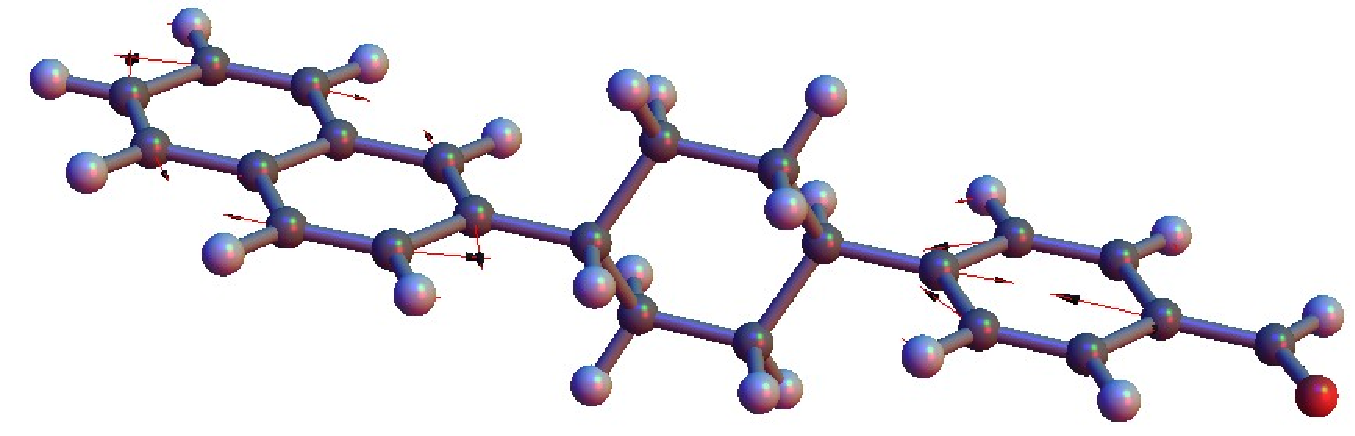
\includegraphics[width=0.75\columnwidth]{Chapters/chap2/Figure4a}}\\
\subfloat[d-2,6ae]{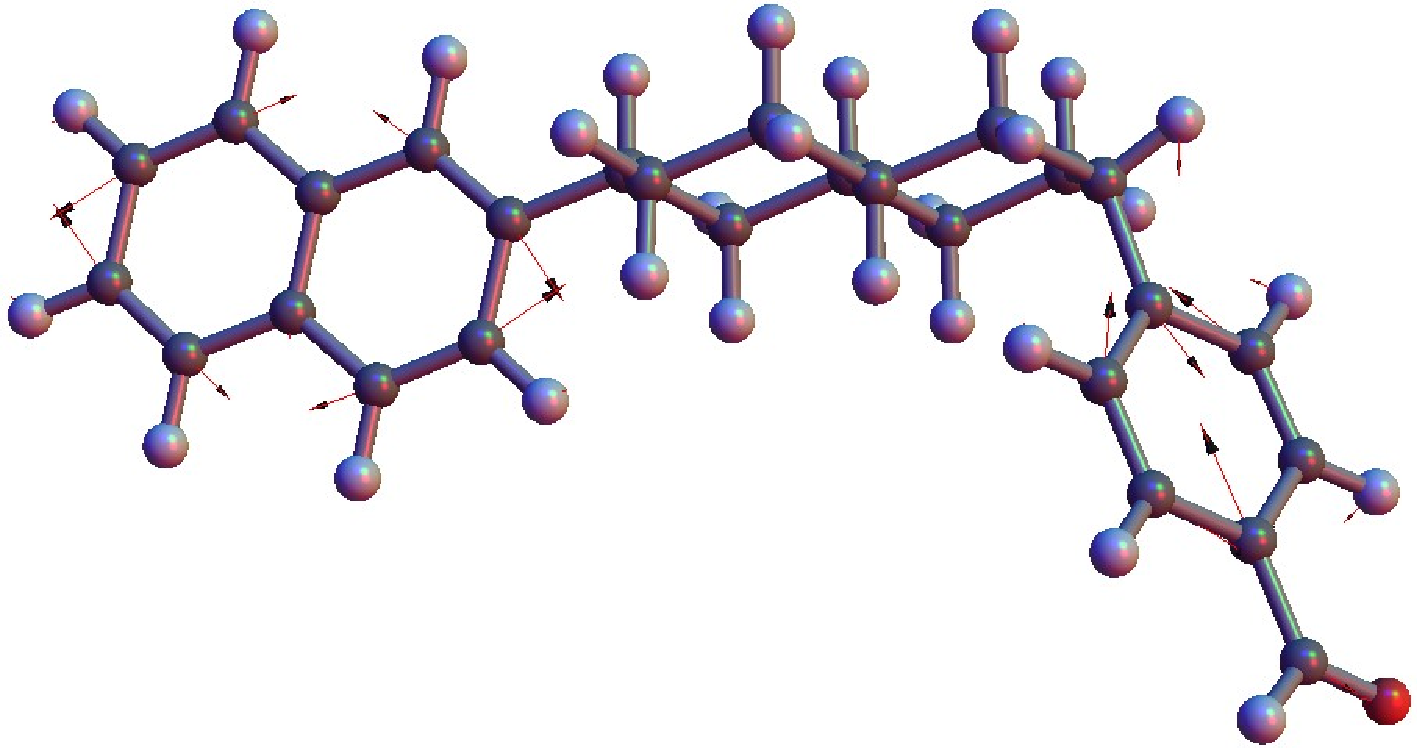
\includegraphics[width=0.75\columnwidth]{Chapters/chap2/Figure4b}}
\caption{
Primary coupling modes for (a) c-1,4ee and (b) d-2,6ae projected onto the atomic displacement coordinates.
}\label{LanczosModes_chap2}
\end{figure}


As an illustrative example of our approach, we consider the
first few collective modes for the c-1,4ee and d-2,5ae cases.
 In Fig.~\ref{LanczosModes_chap2}
we show the projection of the primary coupling mode onto the
coordinate frame of each molecule.  The vectors indicate the direction
of the electron-phonon coupling vectors projected onto the Cartesian displacement
vectors of the individual atoms.   In each case, the primary
coupling mode involves the  $A_{g}$ in plane C=C stretching motions of the naphthalene donor and the
 in-plane $A_1$ ring-squeezing motions of the benzaldehyde acceptor.
It is interesting to note that
% $^{3}B_{2u}$ is also the symmetry of the first triplet $\pi-\pi^{*}$ excited state in naphthalene \cite{aagren1994response}, Moreover,
if we were to approximate naphthalene as a $D_{2h}$ molecule, and benzaldehyde as a $C_{2v}$ molecule, taking the aldehyde as local site, the primary coupling modes always correspond to the totally symmetric irreducible representations on moieties. Further analysis of symmetry reveals interesting details of the reactions, which are discussed in next chapter.
% the resulting first triplet $\pi-\pi^{*}$ is the product of a $b_{1}$ HOMO and a $b_{1}$ LUMO giving a state in the
%   $a_{1}$ irreducible representation. This is the same irreducible representation one obtains for the $\nu_{8}$
%   mode, approximating it as a symmetric stretching mode.
% This suggests the existence of underlying symmetry selection or propensity rule in determining the coupling modes.


In order to substantiate our claim that the reduced modes generated by the iterative
procedure capture the most important electron-phonon couplings, we consider the
convergence of the electron-phonon autocorrelation function used
to compute the golden-rule rate constants
\begin{eqnarray}
C(t) = \langle \hat V_{nm}(t) \hat V_{nm}(0)\rangle \label{c-of-t}
\end{eqnarray}
with respect to the number of reduced modes.  We
calculate  this term exactly using all $N$ vibrational modes of the molecule and
compare to the results obtained using a subset of modes. Correlation function is used to compute transfer rate. Such comparison of correlations is very high standard test of the method. If we get good agreement, it means the reduced modes are a good representation of nuclear motions involved in transfer; even we do not get perfect correlation function, the rate constants calculated may also agree well, which is still a success.


In Fig.~\ref{firstmodecorr}  we examine the convergence of $C(t)$ with respect to number of reduced modes for the c-1,4ee and d-2,6ae cases.
In both cases,  only a handful of reduced modes (4 for c-1,4ee and 15 for d-2,6ae)  is needed to  accurately track the
correlation function for the first 10 fs.   For comparison, d-2,6ae has 162 normal modes and c-1,4ee has 132 normal modes.
For the primary mode approximation, the recursions appear every 23 fs
and are suppressed by the addition of more reduced modes to the calculation.
The 23 fs recursion time corresponds to the period of the single reduced mode: $\omega_{1} = 0.18{\rm eV}$ (1450 cm$^{-1}$).
For the d-2,6ae case, including 15 modes is sufficient to fully suppress the recursion time to  beyond 100 fs.
 For purposes of computing golden rule rate constants,  the Markov limit is reached when
 $C(t)\to 0$.   For the cases at hand, this is well before the first recursion seen in Fig.~\ref{firstmodecorr}.

\begin{figure*}[t]
\subfloat[]{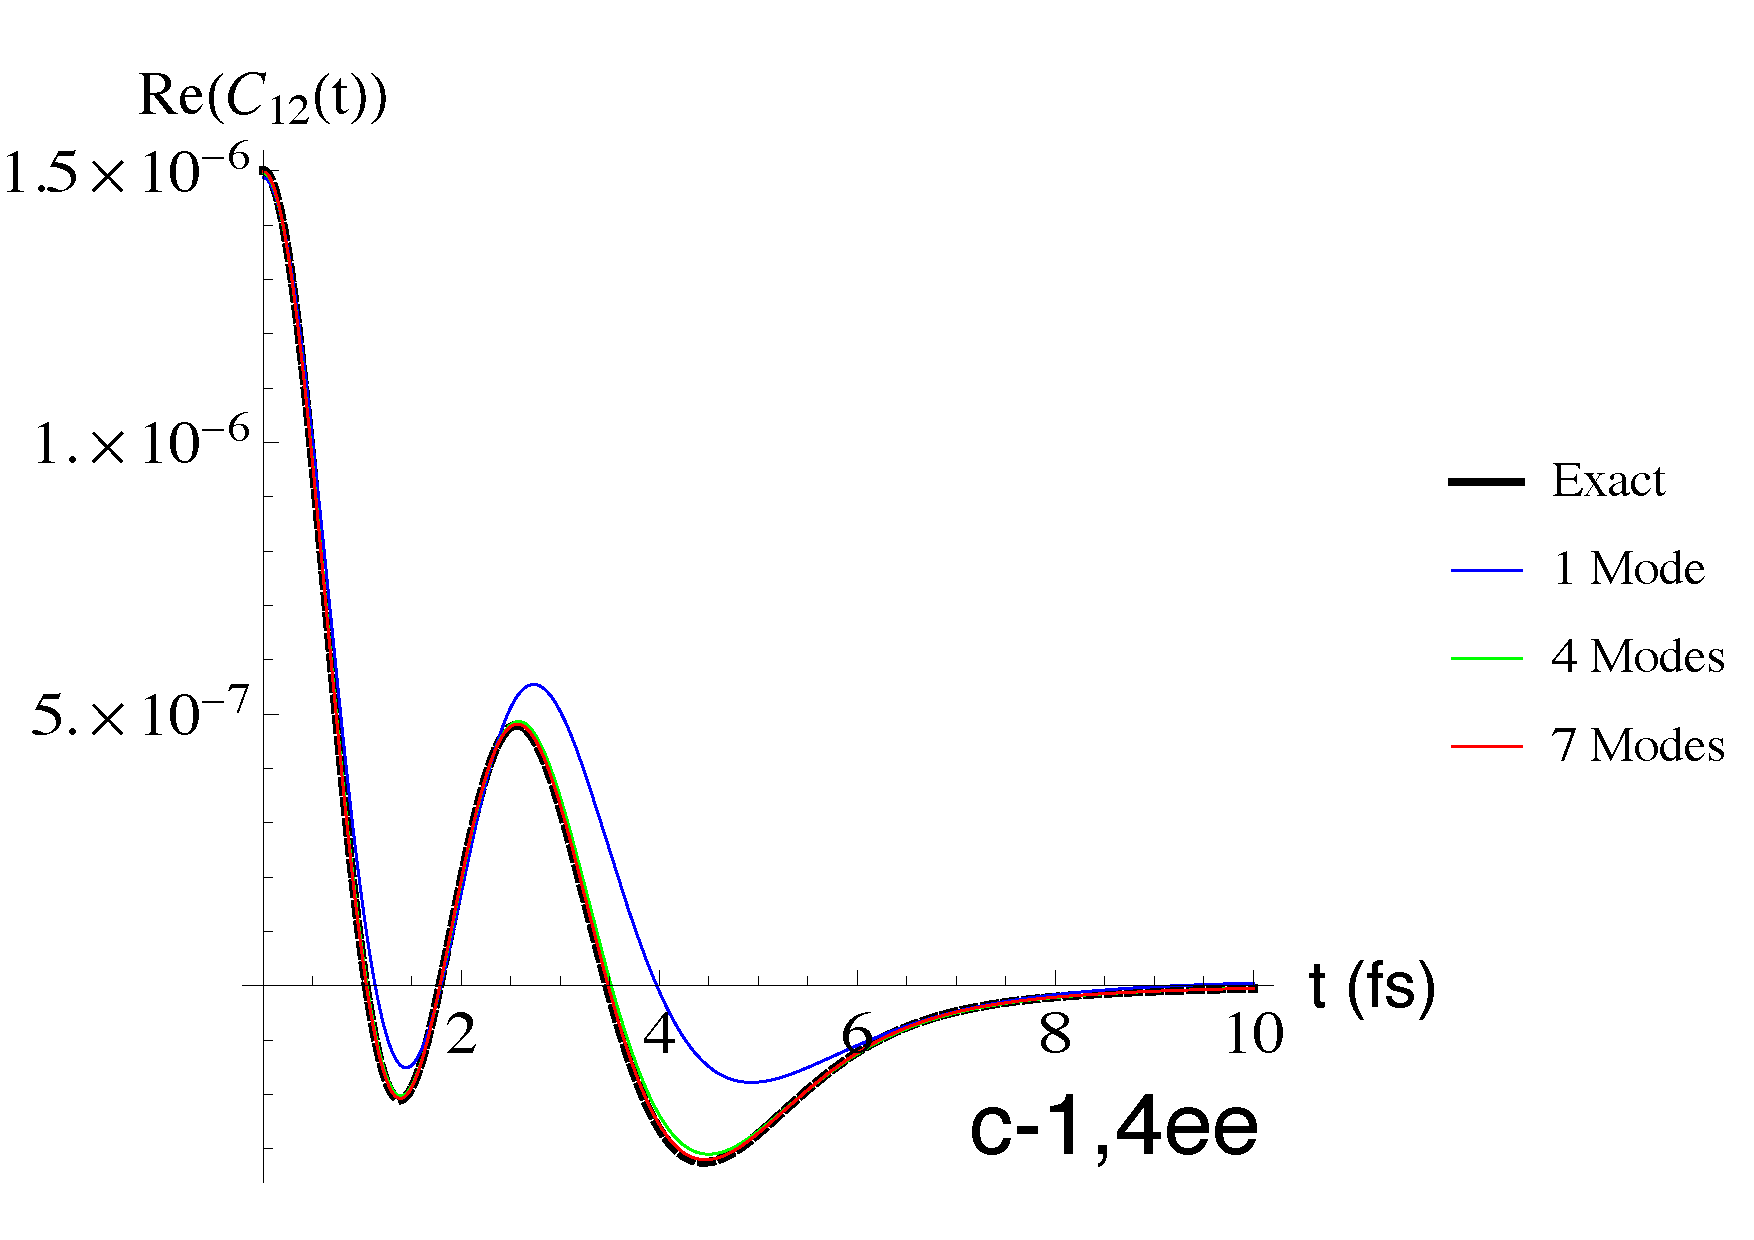
\includegraphics[width=0.45\columnwidth]{Chapters/chap2/Figure5a}}
\subfloat[]{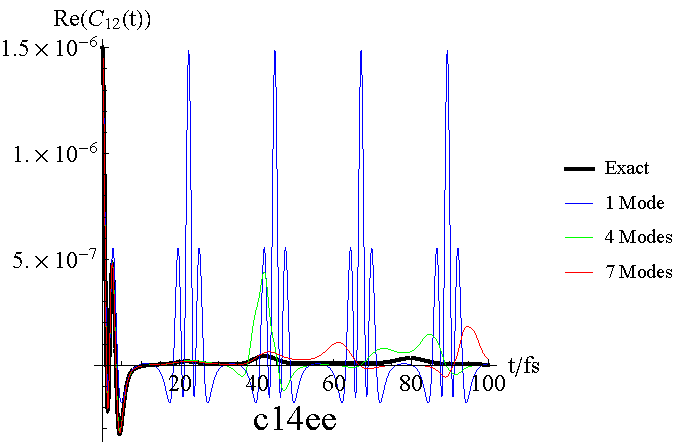
\includegraphics[width=0.45\columnwidth]{Chapters/chap2/Figure5b}}\\
\subfloat[]{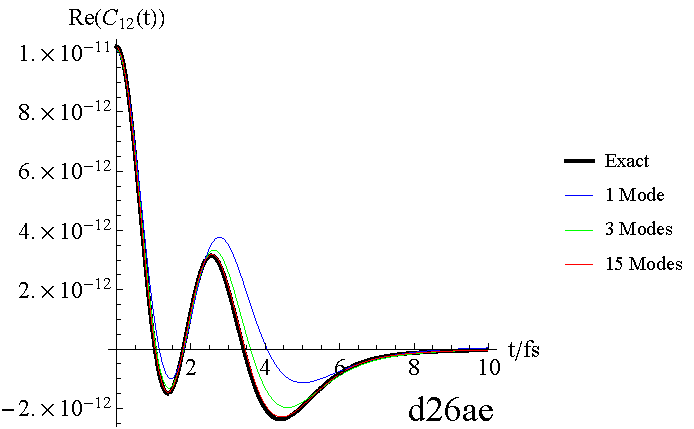
\includegraphics[width=0.45\columnwidth]{Chapters/chap2/Figure5c}}
\subfloat[]{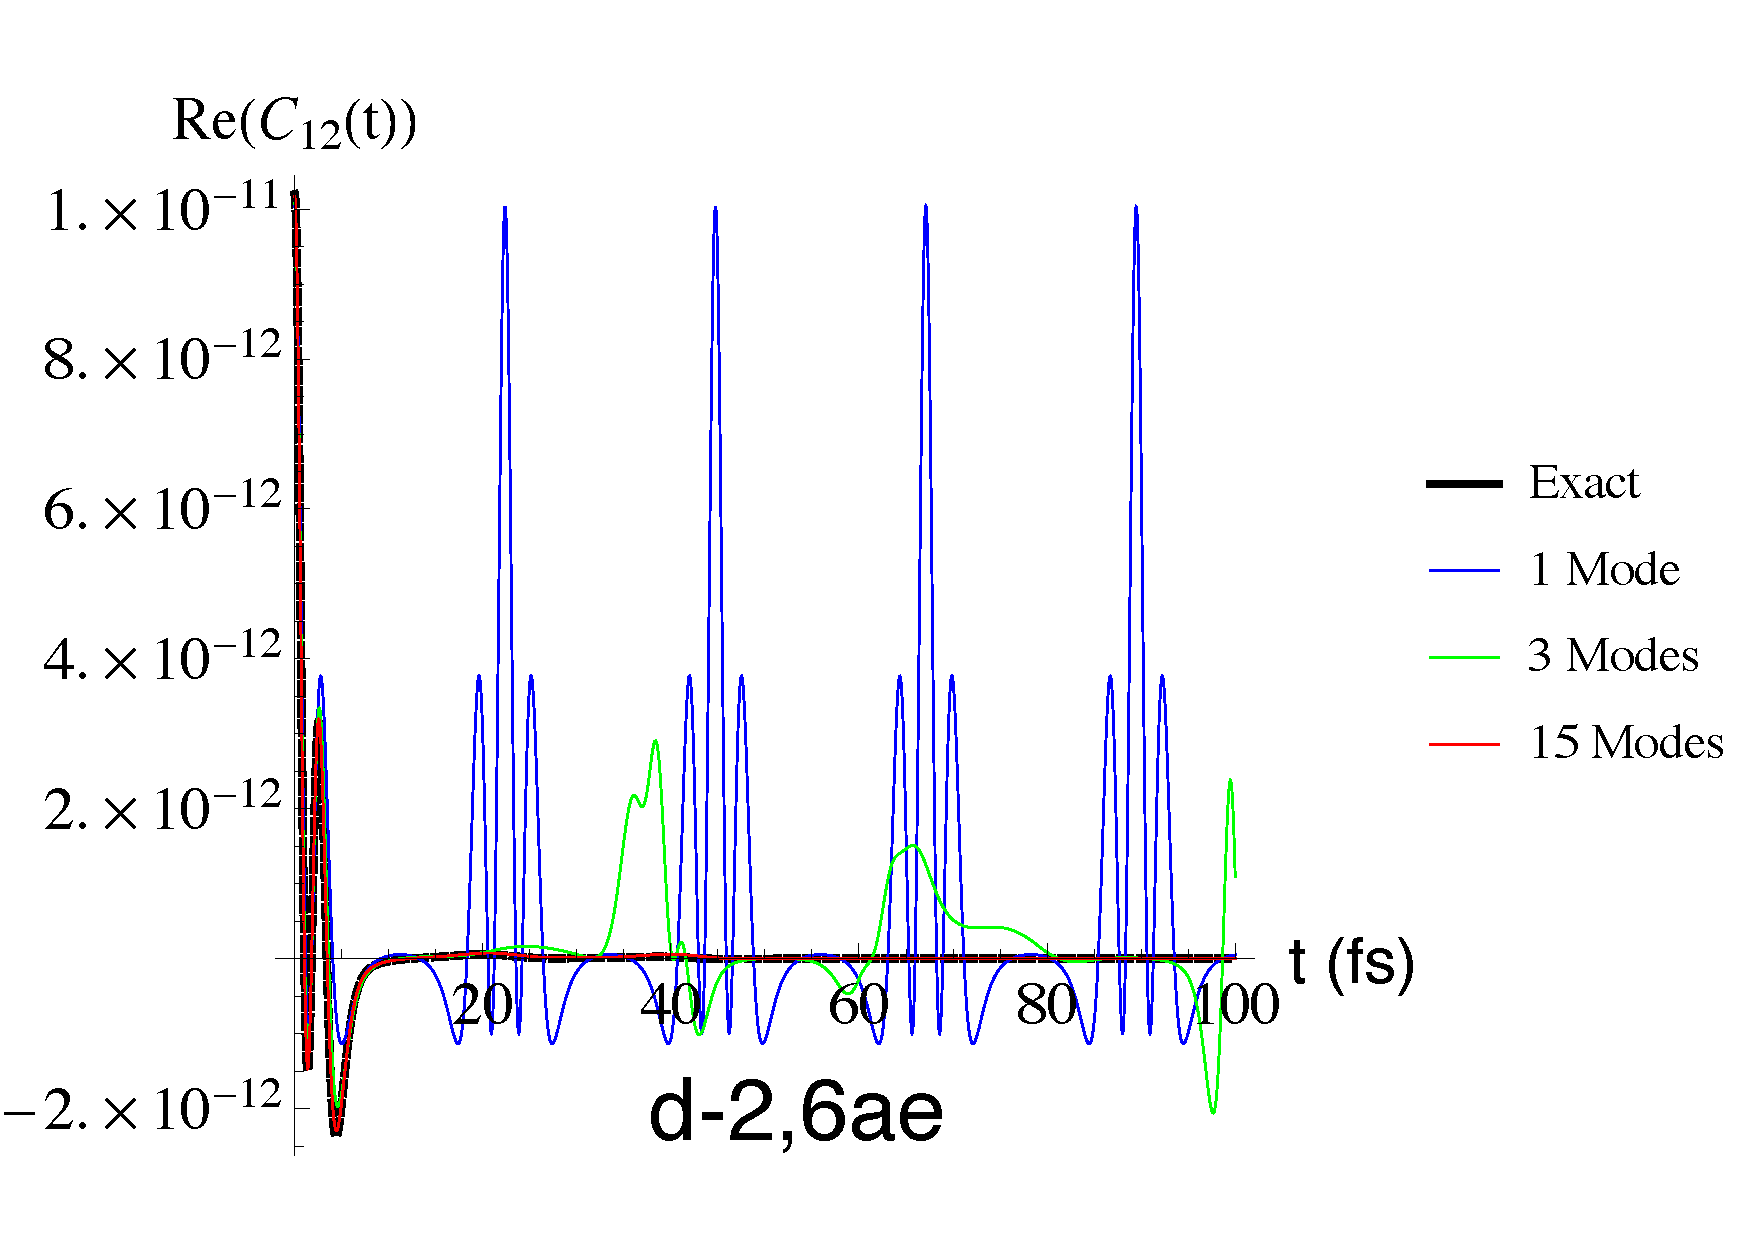
\includegraphics[width=0.45\columnwidth]{Chapters/chap2/Figure5d}}
\caption{Convergence of the electronic coupling autocorrelation function (Eq. ~\ref{c-of-t})
with respect to number of reduced modes.\label{firstmodecorr}}
\end{figure*}

While it is surprising that only a few reduced modes are needed to converge the coupling correlation function, only
a single mode is necessary to accurately compute the golden-rule rate constant.
In Fig.~\ref{fig-1mode} we compare the exact rate constant (using all modes) and rate constants computed using
only the first mode generated by the Lanczos iterations.   In the first case represented by the blue points,
we approximate the renormalized energy as
$$
\lambda_{nm} \approx \frac{g_{1}^{2}}{\omega_1}
$$
where $g_{1}$ and $\omega_{1}$ are the coupling and frequency of the first  reduced mode.  This simple approximation
does a superb job compared to the numerically exact rate obtained using all modes and all couplings.
On average, the error between the exact and approximate rate is 2\%
over the entire series of model donor-bridge-acceptor systems considered.
The red points represent rates computed using the first reduced mode, but use the exact renormalized energy.
Here, the agreement is almost perfect for the two fastest rates corresponding to d-2,6ae and d-2,6ea.   However,  on average
this approximation is off by a factor of 3 compared to the exact rate.  For the methyl-bridged case, the rate is off by a factor of 8..
This implies that the first reduced mode indeed captures the majority of the electron-phonon coupling
 and provides a unique description of the Marcus reaction coordinate.

\begin{figure}[t]
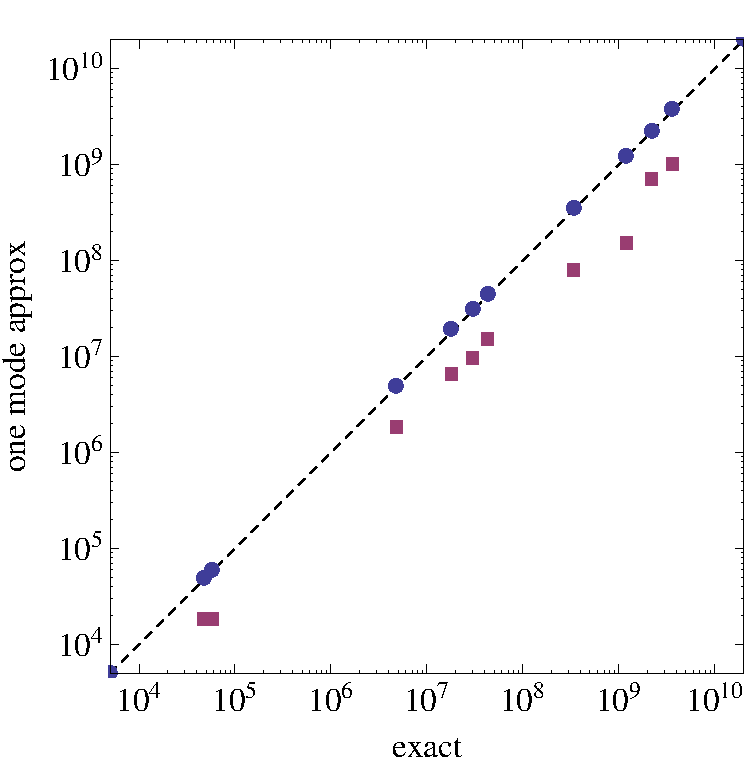
\includegraphics[width=0.6\columnwidth]{Chapters/chap2/Figure6}
\caption{Comparison between exact rate constant and its primary mode approximation.  The blue points correspond to rates computed using
only the primary mode and the renormalized energy for only that mode.  The red points use the primary mode and the exact
renormalized energies. }\label{fig-1mode}
\end{figure}

In Table~\ref{table2} we tabulate the frequencies and electron-phonon coupling constant for the first reduced mode for each
test case.  Uniformly, these modes correspond to ring breathing motions on the donor and acceptor as illustrated in Fig.~\ref{LanczosModes_chap2}.
As seen in this figure, the coupling mode does not involve normal modes localized on the bridge species.
Moreover, the magnitude of the electronic coupling carried by this mode is uniformly around 0.37 eV  and independent of the bridge.
No single normal mode captures all of the electronic coupling.  This is evidenced by the fact that the magnitude of the electronic coupling
carried by the first reduced mode is over twice that of the largest coupling along a single normal mode.



\begin{table}[t]
\centering
\begin{tabular}{lrrr}
 bridge   &  $\omega_1$(eV)  & $|g_{1}|$ (eV)  &  $|g_{max}|$ (eV)  \\
\hline
\hline
 c-1,3ea  &           0.184  &         0.367  &           0.159  \\
 c-1,3ee  &           0.185  &         0.365  &           0.162  \\
 c-1,4ea  &           0.185  &         0.367  &           0.166  \\
 c-1,4ee  &           0.185  &         0.370  &           0.171  \\
 d-2,6ae  &           0.185  &         0.367  &           0.159  \\
 d-2,6ea  &           0.185  &         0.367  &           0.142  \\
 d-2,6ee  &           0.185  &         0.365  &           0.143  \\
 d-2,7ae  &           0.184  &         0.366  &           0.165  \\
 d-2,7ea  &           0.185  &         0.367  &           0.142  \\
 d-2,7ee  &           0.185  &         0.370  &           0.149  \\
 M           &           0.184  &         0.366  &           0.160  \\
 \hline
\end{tabular}
% \end{centering}
\caption{Frequencies and dimensionless electron-phonon couplings for
the primary mode. The last column gives the
absolute value of the largest coupling constant within the normal mode basis.
}\label{table2}

\end{table}


\section{Discussion}

We present here a new approach for computing intramolecular energy and charge transfer rates
by combining a time-convolutionless master equation approach for state to state population transfer as parameterized
by  a rigorous quantum chemical approach.   The approach is robust over a wide range of model systems and
generally gives good agreement compared to experimental rates and Marcus theory rates.
Only in cases where the parabolic approximation to the diabatic potentials breaks down or when the ER localization method
fails to converge is the agreement with the experimental rates less than satisfactory.

A crucial part of our analysis is the identification of a subset of collective modes that contain
the electron-phonon couplings.  Moreover, we show that there exists a unique mode--the ``primary mode'',
determined via an iterative
approach, along which  the off-diagonal electron-phonon coupling is maximized.   Using only the primary mode
mode as input to our golden-rule rate expression, we obtain excellent
agreement (to within 2\% on average over   all of the donor-bridge-acceptor systems studied here)
when compared to an exact evaluation using all normal modes.   One can visualize the primary mode by projecting it on to the
nuclear displacement vectors and gain insight into the coupled electronic/nuclear motions that underlie an electronic
transition.   Our analysis also suggests that the primary  mode resembles certain  irreducible representations of the
donor and acceptor moieties. This connection is further explored in next chapter.

% \begin{}
% \bibliographystyle{chicago}
% \bibliography{Dbib}

% \begin{acknowledgement}

% ERB acknowledges support from
% the National Science Foundation (CHE-1362006), and the Robert A. Welch Foundation (E-1337).
% We specifically thank Prof. Joseph Subotnik and his group for  discussions pertaining to the
% use of the ER localization methods and their implementation in qChem.
% XY thanks Nadia El-Hamdi for inspiration.


% \end{acknowledgement}


% \bibliography{../References-local}
% \bibliographystyle{plainnat}
% \chapterbib
% \providecommand*\mcitethebibliography{\thebibliography}
% \csname @ifundefined\endcsname{endmcitethebibliography}
%   {\let\endmcitethebibliography\endthebibliography}{}
% \begin{mcitethebibliography}{27}
% \providecommand*\natexlab[1]{#1}
% \providecommand*\mciteSetBstSublistMode[1]{}
% \providecommand*\mciteSetBstMaxWidthForm[2]{}
% \providecommand*\mciteBstWouldAddEndPuncttrue
%   {\def\EndOfBibitem{\unskip.}}
% \providecommand*\mciteBstWouldAddEndPunctfalse
%   {\let\EndOfBibitem\relax}
% \providecommand*\mciteSetBstMidEndSepPunct[3]{}
% \providecommand*\mciteSetBstSublistLabelBeginEnd[3]{}
% \providecommand*\EndOfBibitem{}
% \mciteSetBstSublistMode{f}
% \mciteSetBstMaxWidthForm{subitem}{(\alph{mcitesubitemcount})}
% \mciteSetBstSublistLabelBeginEnd
%   {\mcitemaxwidthsubitemform\space}
%   {\relax}
%   {\relax}

% % \begin{thebibliography}{27}
% \bibitem[Marcus(1956)]{marcus1956theory}
% Marcus,~R.~A. On the Theory of Oxidation-Reduction Reactions Involving Electron
%   Transfer. I. \emph{Journal Chem. Phys.} \textbf{1956}, \emph{24},
%   966--978\relax
% \mciteBstWouldAddEndPuncttrue
% \mciteSetBstMidEndSepPunct{\mcitedefaultmidpunct}
% {\mcitedefaultendpunct}{\mcitedefaultseppunct}\relax
% \EndOfBibitem
% \bibitem[Marcus(1965)]{marcus1965theory}
% Marcus,~R.~A. On the Theory of Electron-Transfer Reactions. VI. Unified
%   Treatment for Homogeneous and Electrode Reactions. \emph{J. Chem. Phys} \textbf{1965}, \emph{43}, 679\relax
% \mciteBstWouldAddEndPuncttrue
% \mciteSetBstMidEndSepPunct{\mcitedefaultmidpunct}
% {\mcitedefaultendpunct}{\mcitedefaultseppunct}\relax
% \EndOfBibitem
% \bibitem[Marcus(1993)]{marcus1993electron}
% Marcus,~R.~A. Electron transfer reactions in chemistry. Theory and experiment.
%   \emph{Rev. Mod.  Phys.} \textbf{1993}, \emph{65}, 599--610\relax
% \mciteBstWouldAddEndPuncttrue
% \mciteSetBstMidEndSepPunct{\mcitedefaultmidpunct}
% {\mcitedefaultendpunct}{\mcitedefaultseppunct}\relax
% \EndOfBibitem
% \bibitem[Dexter(1953)]{dexter1953theory}
% Dexter,~D.~L. A Theory of Sensitized Luminescence in Solids. \emph{J. Chem. Phys.} \textbf{1953}, \emph{21}, 836--850\relax
% \mciteBstWouldAddEndPuncttrue
% \mciteSetBstMidEndSepPunct{\mcitedefaultmidpunct}
% {\mcitedefaultendpunct}{\mcitedefaultseppunct}\relax
% \EndOfBibitem
% \bibitem[Miller et~al.(1984)Miller, Calcaterra, and
%   Closs]{miller1984intramolecular}
% Miller,~J.; Calcaterra,~L.; Closs,~G. Intramolecular long-distance electron
%   transfer in radical anions. The effects of free energy and solvent on the
%   reaction rates. \emph{J.  Am.  Chem.  Soc.}
%   \textbf{1984}, \emph{106}, 3047--3049\relax
% \mciteBstWouldAddEndPuncttrue
% \mciteSetBstMidEndSepPunct{\mcitedefaultmidpunct}
% {\mcitedefaultendpunct}{\mcitedefaultseppunct}\relax
% \EndOfBibitem
% \bibitem[Subotnik et~al.(2008)Subotnik, Yeganeh, Cave, and
%   Ratner]{subotnik2008constructing}
% Subotnik,~J.~E.; Yeganeh,~S.; Cave,~R.~J.; Ratner,~M.~A. Constructing diabatic
%   states from adiabatic states: Extending generalized Mulliken--Hush to
%   multiple charge centers with Boys localization. \emph{J. Chem. Phys.} \textbf{2008}, \emph{129}, 244101\relax
% \mciteBstWouldAddEndPuncttrue
% \mciteSetBstMidEndSepPunct{\mcitedefaultmidpunct}
% {\mcitedefaultendpunct}{\mcitedefaultseppunct}\relax
% \EndOfBibitem
% \bibitem[Subotnik et~al.(2009)Subotnik, Cave, Steele, and
%   Shenvi]{subotnik2009initial}
% Subotnik,~J.~E.; Cave,~R.~J.; Steele,~R.~P.; Shenvi,~N. The initial and final
%   states of electron and energy transfer processes: Diabatization as motivated
%   by system-solvent interactions. \emph{J. Chem. Phys.}
%   \textbf{2009}, \emph{130}, 234102--234102\relax
% \mciteBstWouldAddEndPuncttrue
% \mciteSetBstMidEndSepPunct{\mcitedefaultmidpunct}
% {\mcitedefaultendpunct}{\mcitedefaultseppunct}\relax
% \EndOfBibitem
% \bibitem[Subotnik et~al.(2010)Subotnik, Vura-Weis, Sodt, and
%   Ratner]{subotnik2010predicting}
% Subotnik,~J.~E.; Vura-Weis,~J.; Sodt,~A.~J.; Ratner,~M.~A. Predicting accurate
%   electronic energy transfer rates via Marcus theory and Edminston-Ruedeberg
%   localized diabatization. \emph{J. Phys. Chem. A} \textbf{2010},
%   \emph{114}\relax
% \mciteBstWouldAddEndPuncttrue
% \mciteSetBstMidEndSepPunct{\mcitedefaultmidpunct}
% {\mcitedefaultendpunct}{\mcitedefaultseppunct}\relax
% \EndOfBibitem
% \bibitem[Pereverzev and Bittner(2006)Pereverzev, and
%   Bittner]{pereverzev2006time}
% Pereverzev,~A.; Bittner,~E.~R. Time-convolutionless master equation for
%   mesoscopic electron-phonon systems. \emph{J. Chem. Phys.}
%   \textbf{2006}, \emph{125}, 104906\relax
% \mciteBstWouldAddEndPuncttrue
% \mciteSetBstMidEndSepPunct{\mcitedefaultmidpunct}
% {\mcitedefaultendpunct}{\mcitedefaultseppunct}\relax
% \EndOfBibitem
% \bibitem[Tamura et~al.(2008)Tamura, Ramon, Bittner, and Burghardt]{tamura2008phonon}
% Tamura,~H.; Ramon,~J. G.~S.; Bittner,~E.~R.; Burghardt,~I. Phonon-Driven
%   Ultrafast Exciton Dissociation at Donor-Acceptor Polymer Heterojunctions.
%   \emph{Physical Review Letters} \textbf{2008}, \emph{100}, APS\relax
% \mciteBstWouldAddEndPuncttrue
% \mciteSetBstMidEndSepPunct{\mcitedefaultmidpunct}
% {\mcitedefaultendpunct}{\mcitedefaultseppunct}\relax
% \EndOfBibitem
% \bibitem[Tamura et~al.(2007)Tamura, Bittner, and Burghardt]{tamura2007exciton}
% Tamura,~H.; Bittner,~E.~R.; Burghardt,~I. Exciton dissociation at
%   donor-acceptor polymer heterojunctions: Quantum nonadiabatic dynamics and
%   effective-mode analysis. \emph{J. Chem. Phys.}
%   \textbf{2007}, \emph{126}, 021103\relax
% \mciteBstWouldAddEndPuncttrue
% \mciteSetBstMidEndSepPunct{\mcitedefaultmidpunct}
% {\mcitedefaultendpunct}{\mcitedefaultseppunct}\relax
% \EndOfBibitem
% \bibitem[Bittner and Silva(2014)Bittner, and Silva]{bittner2014noise}
% Bittner,~E.~R.; Silva,~C. Noise-induced quantum coherence drives photo-carrier
%   generation dynamics at polymeric semiconductor heterojunctions. \emph{Nat.   Comm.} \textbf{2014}, \emph{5}, 3119\relax
% \mciteBstWouldAddEndPuncttrue
% \mciteSetBstMidEndSepPunct{\mcitedefaultmidpunct}
% {\mcitedefaultendpunct}{\mcitedefaultseppunct}\relax
% \EndOfBibitem
% \bibitem[Singh et~al.(2009)Singh, Bittner, Beljonne, and
%   Scholes]{singh2009fluorescence}
% Singh,~J.; Bittner,~E.~R.; Beljonne,~D.; Scholes,~G.~D. Fluorescence Depolarization in MEH-PPV:
% Sites vs. Eigenstates Hopping. \emph{J. Chem.
%   Phys.} \textbf{2009}, \emph{131}, 194905\relax
% \mciteBstWouldAddEndPuncttrue
% \mciteSetBstMidEndSepPunct{\mcitedefaultmidpunct}
% {\mcitedefaultendpunct}{\mcitedefaultseppunct}\relax
% \EndOfBibitem
% \bibitem[Cederbaum et~al.(2005)Cederbaum, Gildensperger, and
%   Burghardt]{cederbaum2005short}
% Cederbaum,~L.; Gildensperger,~E.; Burghardt,~I. Short-Time Dynamics Through
%   Conical Intersections in Macrosystems. \emph{Phys. Rev. Lett.} \textbf{2005},
%   \emph{94}, 113003\relax
% \mciteBstWouldAddEndPuncttrue
% \mciteSetBstMidEndSepPunct{\mcitedefaultmidpunct}
% {\mcitedefaultendpunct}{\mcitedefaultseppunct}\relax
% \EndOfBibitem
% \bibitem[Gindensperger et~al.(2006)Gindensperger, Burghardt, and
%   Cederbaum]{gindensperger2006shortI}
% Gindensperger,~E.; Burghardt,~I.; Cederbaum,~L.~S. Short-time dynamics through
%   conical intersections in macrosystems. I. Theory: Effective-mode formulation.
%   \emph{J. Chem. Phys.} \textbf{2006}, \emph{124},
%   144103\relax
% \mciteBstWouldAddEndPuncttrue
% \mciteSetBstMidEndSepPunct{\mcitedefaultmidpunct}
% {\mcitedefaultendpunct}{\mcitedefaultseppunct}\relax
% \EndOfBibitem
% \bibitem[Gindensperger et~al.(2006)Gindensperger, Burghardt, and
%   Cederbaum]{gindensperger2006shortII}
% Gindensperger,~E.; Burghardt,~I.; Cederbaum,~L.~S. Short-time dynamics through
%   conical intersections in macrosystems. II. Applications. \emph{J. Chem. Phys.} \textbf{2006}, \emph{124}, 144104\relax
% \mciteBstWouldAddEndPuncttrue
% \mciteSetBstMidEndSepPunct{\mcitedefaultmidpunct}
% {\mcitedefaultendpunct}{\mcitedefaultseppunct}\relax
% \EndOfBibitem
% \bibitem[Cederbaum et~al.(2005)Cederbaum, Gindensperger, and
%   Burghardt]{cederbaum2005short}
% Cederbaum,~L.~S.; Gindensperger,~E.; Burghardt,~I. Short-Time Dynamics Through
%   Conical Intersections in Macrosystems. \emph{Phys. Rev. Lett.} \textbf{2005},
%   \emph{94}, 113003\relax
% \mciteBstWouldAddEndPuncttrue
% \mciteSetBstMidEndSepPunct{\mcitedefaultmidpunct}
% {\mcitedefaultendpunct}{\mcitedefaultseppunct}\relax
% \EndOfBibitem
% \bibitem[Pereverzev et~al.(2009)Pereverzev, Bittner, and  Burghardt]{pereverzev2009energy}
% Pereverzev,~A.; Bittner,~E.~R.; Burghardt,~I. Energy and charge-transfer
%   dynamics using projected modes. \emph{J. Chem. Phys.}
%   \textbf{2009}, \emph{131}, 034104\relax
% \mciteBstWouldAddEndPuncttrue
% \mciteSetBstMidEndSepPunct{\mcitedefaultmidpunct}
% {\mcitedefaultendpunct}{\mcitedefaultseppunct}\relax
% \EndOfBibitem
% \bibitem[Closs et~al.(1988)Closs, Piotrowiak, MacInnis, and
%   Fleming]{closs1988determination}
% Closs,~G.~L.; Piotrowiak,~P.; MacInnis,~J.~M.; Fleming,~G.~R. Determination of
%   long-distance intramolecular triplet energy-transfer rates. Quantitative
%   comparison with electron transfer. \emph{J.  Am.  Chem.  Soc.} \textbf{1988}, \emph{110}, 2652--2653\relax
% \mciteBstWouldAddEndPuncttrue
% \mciteSetBstMidEndSepPunct{\mcitedefaultmidpunct}
% {\mcitedefaultendpunct}{\mcitedefaultseppunct}\relax
% \EndOfBibitem
% \bibitem[Closs et~al.(1989)Closs, Johnson, Miller, and
%   Piotrowiak]{closs1989connection}
% Closs,~G.~L.; Johnson,~M.~D.; Miller,~J.~R.; Piotrowiak,~P. A connection
%   between intramolecular long-range electron, hole, and triplet energy
%   transfers. \emph{J.  Am.  Chem.  Soc.} \textbf{1989},
%   \emph{111}, 3751--3753\relax
% \mciteBstWouldAddEndPuncttrue
% \mciteSetBstMidEndSepPunct{\mcitedefaultmidpunct}
% {\mcitedefaultendpunct}{\mcitedefaultseppunct}\relax
% \EndOfBibitem
% \bibitem[Grover and Silbey(1970)Grover, and Silbey]{grover1970exciton}
% Grover,~M.~K.; Silbey,~R. Exciton--Phonon Interactions in Molecular Crystals.
%   \emph{J. Chem. Phys.} \textbf{1970}, \emph{52},
%   2099--2108\relax
% \mciteBstWouldAddEndPuncttrue
% \mciteSetBstMidEndSepPunct{\mcitedefaultmidpunct}
% {\mcitedefaultendpunct}{\mcitedefaultseppunct}\relax
% \EndOfBibitem
% \bibitem[Rice and Gartstein(1994)Rice, and Gartstein]{rice1994excitons}
% Rice,~M.~J.; Gartstein,~Y.~N. Excitons and interband excitations in conducting
%   polymers based on phenylene. \emph{Phys. Rev. Lett.} \textbf{1994},
%   \emph{73}, 2504--2507\relax
% \mciteBstWouldAddEndPuncttrue
% \mciteSetBstMidEndSepPunct{\mcitedefaultmidpunct}
% {\mcitedefaultendpunct}{\mcitedefaultseppunct}\relax
% \EndOfBibitem
% \bibitem[Edmiston and Ruedenberg(1963)Edmiston, and
%   Ruedenberg]{edmiston1963localized}
% Edmiston,~C.; Ruedenberg,~K. Localized Atomic and Molecular Orbitals.
%   \emph{Rev. Mod. Phys.} \textbf{1963}, \emph{35}, 457--464\relax
% \mciteBstWouldAddEndPuncttrue
% \mciteSetBstMidEndSepPunct{\mcitedefaultmidpunct}
% {\mcitedefaultendpunct}{\mcitedefaultseppunct}\relax
% \EndOfBibitem
% \bibitem[Closs and Miller(1988)Closs, and Miller]{closs1988intramolecular}
% Closs,~G.~L.; Miller,~J.~R. Intramolecular long-distance electron transfer in
%   organic molecules. \emph{Science} \textbf{1988}, \emph{240}, 440--447\relax
% \mciteBstWouldAddEndPuncttrue
% \mciteSetBstMidEndSepPunct{\mcitedefaultmidpunct}
% {\mcitedefaultendpunct}{\mcitedefaultseppunct}\relax
% \EndOfBibitem
% \bibitem[Silva and Reilly(1996)Silva, and Reilly]{silva1996theoretical}
% Silva,~C.~R.; Reilly,~J.~P. Theoretical Calculations on Excited Electronic
%   States of Benzaldehyde and Observation of the $S_2\leftarrow S_0$ Jet-Cooled
%   Spectrum. \emph{J. Phys. Chem.} \textbf{1996}, \emph{100},
%   17111--17123\relax
% \mciteBstWouldAddEndPuncttrue
% \mciteSetBstMidEndSepPunct{\mcitedefaultmidpunct}
% {\mcitedefaultendpunct}{\mcitedefaultseppunct}\relax
% \EndOfBibitem
% \bibitem[{\AA}gren et~al.(1994){\AA}gren, Minaev, and
%   Knuts]{aagren1994response}
% {\AA}gren,~H.; Minaev,~B.~F.; Knuts,~S. Response Theory Studies of
%   Triplet-State Spectra and Radiative Lifetimes of Naphthalene, Quinoxaline,
%   and Phthalazine. \emph{J.  Phys.  Chem.} \textbf{1994},
%   \emph{98}, 3943--3949\relax
% \mciteBstWouldAddEndPuncttrue
% \mciteSetBstMidEndSepPunct{\mcitedefaultmidpunct}
% {\mcitedefaultendpunct}{\mcitedefaultseppunct}\relax
% \EndOfBibitem

% % \end{thebibliography}
% \end{mcitethebibliography}

% \begin{tocentry}
% {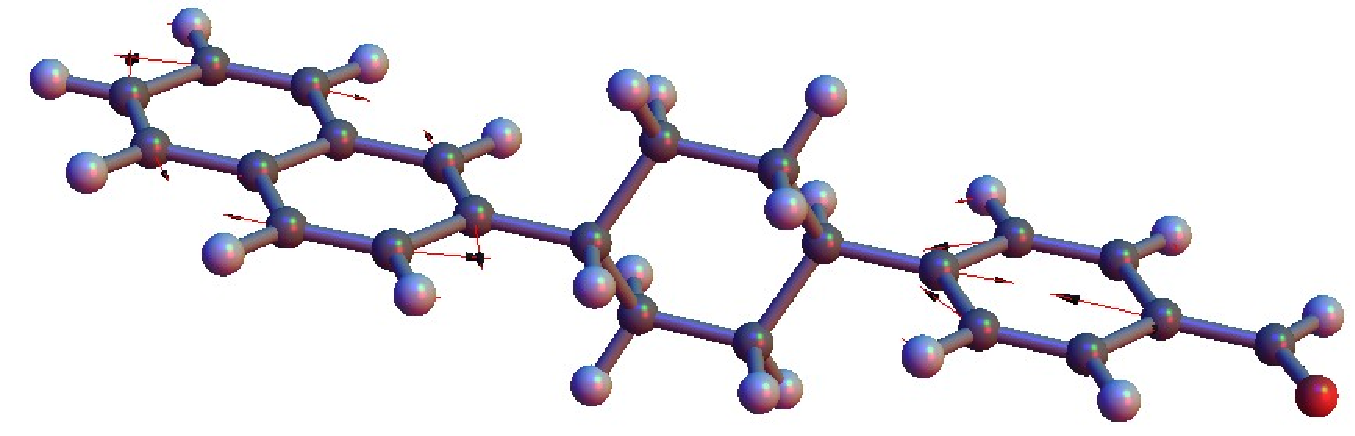
\includegraphics[width=4.3cm]{Chapters/chap2/TOCFigure1}}
% {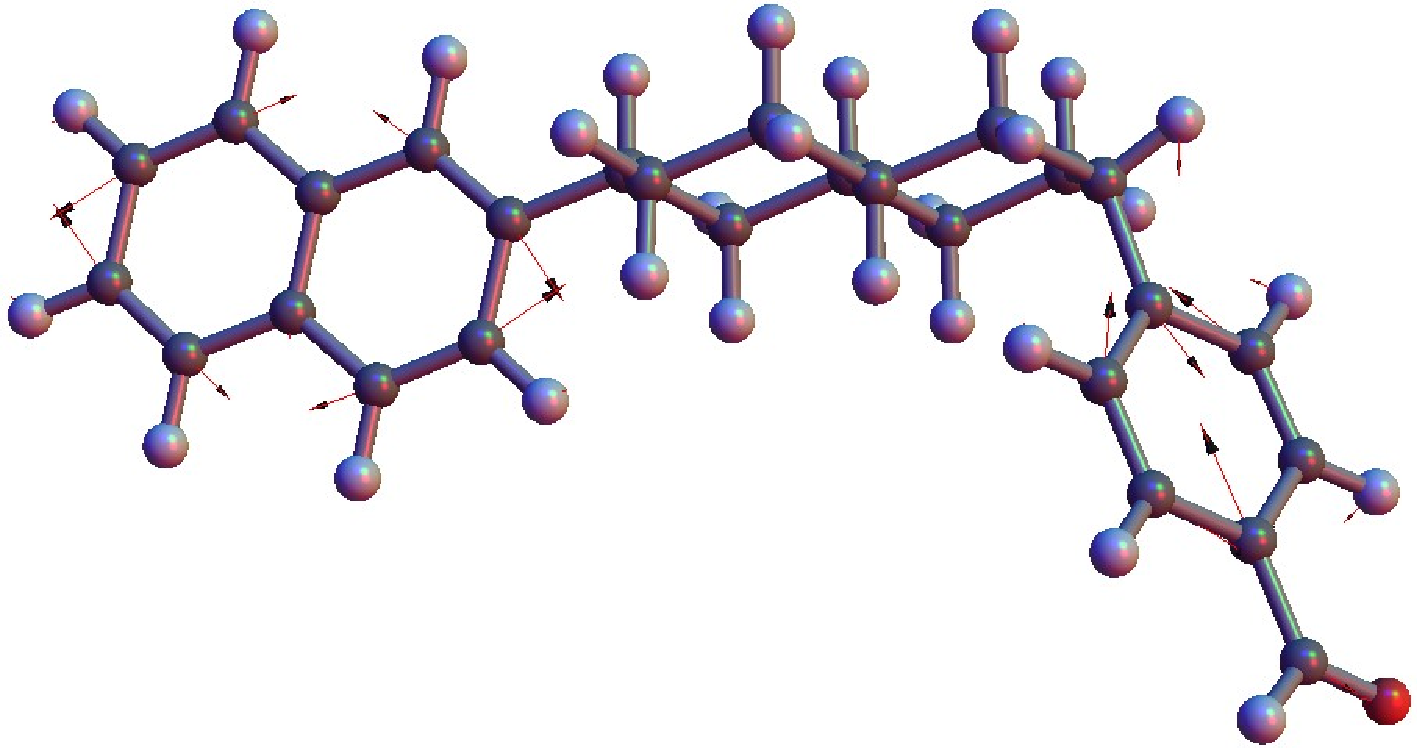
\includegraphics[width=4.3cm]{Chapters/chap2/TOCFigure2}}
% %Primary coupling modes for triplet energy transfer in model donor-bridge-acceptor systems.
% %These modes provide a unique representation of the electron/nuclear coupling for intramolecular charge and energy-transfer.
% \end{tocentry}




% \end{document}
